%  LaTeX support: latex@mdpi.com 
%  For support, please attach all files needed for compiling as well as the log file, and specify your operating system, LaTeX version, and LaTeX editor.

%=================================================================
\documentclass[notspecified,article,submit,pdftex,moreauthors]{Definitions/mdpi}
%\documentclass[preprints,article,submit,pdftex,moreauthors]{Definitions/mdpi}
% For posting an early version of this manuscript as a preprint, you may use "preprints" as the journal. Changing "submit" to "accept" before posting will remove line numbers.

%--------------------
% Class Options:
%--------------------
%----------
% journal
%----------
% Choose between the following MDPI journals:
% accountaudit, acoustics, actuators, addictions, adhesives, adolescents, aerobiology, aerospace, agriculture, agriengineering, agrochemicals, agronomy, ai, aichem, aieng, aimater, aimed, aipa, air, aisens, algorithms, allergies, alloys, amh, analog, analytica, analytics, anatomia, anesthres, animals, antibiotics, antibodies, antioxidants, applbiosci, appliedchem, appliedmath, appliedphys, applmech, applmicrobiol, applnano, applsci, aquacj, architecture, arm, arthropoda, asc, asi, astronautics, astronomy, atmosphere, atoms, audiolres, automation, axioms, bacteria, batteries, bdcc, beverages, biochem, bioengineering, biologics, biology, biomass, biomechanics, biomed, biomedicines, biomedinformatics, biomimetics, biomolecules, biophysica, bioresourbioprod, biosensors, biosphere, biotech, birds, blockchains, bloods, blsf, brainsci, breath, buildings, cancers, carbon, cardio, cardiogenetics, cardiovascmed, catalysts, cells, ceramics, challenges, chemengineering, chemistry, chemosensors, chemproc, children, chips, cimb, civileng, cleantechnol, climate, clinbioenerg, clinpract, clockssleep, cmd, cmtr, coasts, coatings, colloids, colorants, commodities, complexities, complications, compounds, computation, computers, condensedmatter, conservation, constrmater, cosmetics, covid, crops, cryo, cryptography, crystals, csmf, ctn, culture, curroncol, cyber, dairy, data, ddc, dentistry, dermato, dermatopathology, designs, devices, dhi, diabetology, diagnostics, dietetics, digital, disabilities, diseases, diversity, dna, drones, dynamics, earth, ebj, ecm, ecologies, edm, eesp, electricity, electrochem, electronicmat, electronics, encyclopedia, endocrines, energies, eng, engproc, entomology, entropy, environments, environremediat, epidemiologia, epigenomes, esa, est, fermentation, fibers, fintech, fire, fishes, fluids, foods, forecasting, forensicsci, forests, fossstud, foundations, fractalfract, fuels, future, futureinternet, futurepharmacol, futurephys, futuretransp, galaxies, gases, gastroent, gastrointestdisord, gastronomy, gels, genes, geographies, geohazards, geomatics, geometry, geosciences, geotechnics, geriatrics, germs, glacies, grasses, green, greenhealth, gucdd, hardware, hazardousmatters, healthcare, hearts, hemato, hematolrep, hep, heritage, higheredu, highthroughput, horticulturae, hospitals, hydrobiology, hydrogen, hydrology, hydropower, hygiene, idr, iic, ijem, ijerph, ijgi, ijmd, ijms, ijns, ijom, ijpb, ijt, ijtm, ijtpp, ime, immuno, informatics, information, infrastructures, inorganics, insects, instruments, inventions, iot, j, jaestheticmed, jal, jcdd, jcm, jcp, jcrm, jcs, jcto, jdad, jdb, jdream, jemr, jeta, jfb, jfmk, jgbg, jgg, jimaging, jlpea, jmahp, jmmp, jmms, jmp, jmse, jne, jnt, jof, joi, joitmc, joma, jop, joptm, jor, jox, jpbi, jytomed, jpm, jsan, jtaer, jvd, jzbg, kidneydial, kinasesphosphatases, knowledge, labmed, laboratories, lae, land, life, lights, limnolrev, lipidology, liquids, livers, logics, logistics, lubricants, lymphatics, machines, macromol, magnetism, magnetochemistry, make, marinedrugs, materials, materproc, mathematics, mca, measurements, medicina, medicines, medsci, membranes, merits, metabolites, metals, meteorology, methane, metrics, metrology, micro, microarrays, microbiolres, microelectronics, micromachines, microorganisms, microplastics, microwave, minerals, mining, mmphys, modelling, molbank, molecules, mps, msf, mti, multimedia, muscles, nanoenergyadv, nanomanufacturing, nanomaterials, ncrna, ndt, network, neuroglia, neuroimaging, neurolint, neurosci, nitrogen, notspecified, nursrep, nutraceuticals, nutrients, obesities, occuphealth, oceans, ohbm, onco, optics, oral, organics, organoids, osteology, oxygen, pandemics, parasites, parasitologia, particles, pathogens, pathophysiology, pediatrrep, pets, pharmaceuticals, pharmaceutics, pharmacoepidemiology, pharmacy, philosophies, photochem, photonics, phycology, physchem, physics, physiologia, plants, plasma, platforms, pollutants, polymers, polysaccharides, populations, poultry, powders, precipitation, precisoncol, preprints, proceedings, processes, prosthesis, proteomes, psf, psychiatryint, psychoactives, purification, quantumrep, quaternary, qubs, radiation, rdt, reactions, realestate, receptors, recycling, regeneration, remotesensing, reports, reprodmed, resources, rheumato, rjpm, robotics, rsee, ruminants, safety, sci, scipharm, sclerosis, seeds, sensors, separations, sexes, shi, signals, sinusitis, siuj, skins, smartcities, sna, societies, software, soilsystems, solar, solids, spectroscj, sports, standards, stats, std, stratsediment, stresses, surfaces, surgeries, suschem, sustainability, symmetry, synbio, systems, tae, targets, taxonomy, technologies, telecom, test, textiles, thalassrep, therapeutics, thermo, timespace, tomography, toxics, toxins, tph, transplantology, transportation, traumacare, traumas, tri, tropicalmed, universe, urbansci, uro, vaccines, vehicles, venereology, vetsci, vibration, virtualworlds, viruses, vision, waste, water, welding, wem, wevj, wild, wind, women, world, zoonoticdis

%---------
% article
%---------
% The default type of manuscript is "article", but can be replaced by: 
% abstract, addendum, article, benchmark, book, bookreview, briefcommunication, briefreport, casereport, changes, clinicopathologicalchallenge, comment, commentary, communication, conceptpaper, conferenceproceedings, correction, conferencereport, creative, datadescriptor, discussion, entry, expressionofconcern, extendedabstract, editorial, essay, erratum, fieldguide, hypothesis, interestingimages, letter, meetingreport, monograph, newbookreceived, obituary, opinion, proceedingpaper, projectreport, reply, retraction, review, perspective, protocol, shortnote, studyprotocol, supfile, systematicreview, technicalnote, viewpoint, guidelines, registeredreport, tutorial,  giantsinurology, urologyaroundtheworld
% supfile = supplementary materials

%----------
% submit
%----------
% The class option "submit" will be changed to "accept" by the Editorial Office when the paper is accepted. This will only make changes to the frontpage (e.g., the logo of the journal will get visible), the headings, and the copyright information. Also, line numbering will be removed. Journal info and pagination for accepted papers will also be assigned by the Editorial Office.

%------------------
% moreauthors
%------------------
% If there is only one author the class option oneauthor should be used. Otherwise use the class option moreauthors.

%---------
% pdftex
%---------
% The option pdftex is for use with pdfLaTeX. Remove "pdftex" for (1) compiling with LaTeX & dvi2pdf (if eps figures are used) or for (2) compiling with XeLaTeX.

%=================================================================
% MDPI internal commands - do not modify
\firstpage{1} 
\makeatletter 
\setcounter{page}{\@firstpage} 
\makeatother
\pubvolume{1}
\issuenum{1}
\articlenumber{0}
\pubyear{2026}
\copyrightyear{2026}
%\externaleditor{Firstname Lastname} % More than 1 editor, please add `` and '' before the last editor name
\datereceived{ } 
\daterevised{ } % Comment out if no revised date
\dateaccepted{ } 
\datepublished{ } 
%\datecorrected{} % For corrected papers: "Corrected: XXX" date in the original paper.
%\dateretracted{} % For retracted papers: "Retracted: XXX" date in the original paper.
%\doinum{} % Used for some special journals, like molbank
%\pdfoutput=1 % Uncommented for upload to arXiv.org
%\CorrStatement{yes}  % For updates
%\longauthorlist{yes} % For many authors that exceed the left citation part
%\IsAssociation{yes} % For association journals
\setlength{\headheight}{20pt}

%=================================================================
% Add packages and commands here. The following packages are loaded in our class file: fontenc, inputenc, calc, indentfirst, fancyhdr, graphicx, epstopdf, lastpage, ifthen, float, amsmath, amssymb, lineno, setspace, enumitem, mathpazo, booktabs, titlesec, etoolbox, tabto, xcolor, colortbl, soul, multirow, microtype, tikz, totcount, changepage, attrib, upgreek, array, tabularx, pbox, ragged2e, tocloft, marginnote, marginfix, enotez, amsthm, natbib, hyperref, cleveref, scrextend, url, geometry, newfloat, caption, draftwatermark, seqsplit
% cleveref: load \crefname definitions after \begin{document}

%=================================================================
% Please use the following mathematics environments: Theorem, Lemma, Corollary, Proposition, Characterization, Property, Problem, Example, ExamplesandDefinitions, Hypothesis, Remark, Definition, Notation, Assumption
% For proofs, please use the proof environment (the amsthm package is loaded by the MDPI class).

%=================================================================
% Full title of the paper (Capitalized)
\Title{MARL-based Trust Evaluation for Zero-Trust Low-Altitude UAV Networks}

% Author Orchid ID: enter ID or remove command
\newcommand{\orcidauthorA}{0000-0000-0000-000X} % Add \orcidA{} behind the author's name
%\newcommand{\orcidauthorB}{0000-0000-0000-000X} % Add \orcidB{} behind the author's name

% Authors, for the paper (add full first names)
\Author{Firstname Lastname $^{1}$\orcidA{}, Firstname Lastname $^{2}$ and Firstname Lastname $^{2,}$*}

%\longauthorlist{yes}

% MDPI internal command: Authors, for metadata in PDF
\AuthorNames{Firstname Lastname, Firstname Lastname and Firstname Lastname}

% Affiliations / Addresses (Add [1] after \address if there is only one affiliation.)
\address{%
$^{1}$ \quad Affiliation 1; e-mail@e-mail.com\\
$^{2}$ \quad Affiliation 2; e-mail@e-mail.com}

% Contact information of the corresponding author
\corres{Correspondence: e-mail@e-mail.com; Tel.: (optional; include country code; if there are multiple corresponding authors, add author initials) +xx-xxxx-xxx-xxxx (F.L.)}

% Current address and/or shared authorship
%\firstnote{Current address: Affiliation.}  
% Current address should not be the same as any items in the Affiliation section.

%\secondnote{These authors contributed equally to this work.}
% The commands \thirdnote{} till \eighthnote{} are available for further notes.

%\simplesumm{} % Simple summary

%\conference{} % An extended version of a conference paper

% Abstract (Do not insert blank lines, i.e. \\) 
\abstract{Low-altitude UAV networks face significant security challenges due to rapidly changing topology, intermittent links, and limited onboard resources, making them vulnerable to spoofing, tampering, and collusive attacks. Existing trust evaluation schemes often suffer from degraded detection accuracy under high malicious-node ratios because they rely on static trust weighting or centralized coordination. To address these limitations, this paper proposes MTIM, a Multi-agent Reinforcement Learning-based Trust Evaluation Mechanism for zero-trust low-altitude UAV networks. MTIM integrates five complementary trust dimensions with cross-factor consistency checking, distributed trust learning via Thinker Agents, Bayesian uncertainty-aware aggregation through an Inferential Conclusion Agent, and temporally decayed state updates. Simulation results demonstrate that MTIM achieves a detection accuracy of 93.0\% and a task success rate of 90.0\% under a 30\% malicious-node ratio, outperforming GDM-DTM by 10.6 percentage points in accuracy and consistently exceeding all compared baselines. These results confirm that combining multi-factor evidence with MARL-based adaptive weighting significantly improves robustness and mission-level decision quality in dynamic zero-trust UAV environments.}

% Keywords
\keyword{UAV networks; trust management; multi-agent reinforcement learning; zero trust architecture; FANET security}   
  
% The fields PACS, MSC, and JEL may be left empty or commented out if not applicable
%\PACS{J0101}
%\MSC{}
%\JEL{}

%%%%%%%%%%%%%
% Only for the journal Diversity
%\LSID{\url{http://}}

%%%%%%%%%%%%%
% Only for the journal Applied Sciences
%\featuredapplication{Authors are encouraged to provide a concise description of the specific application or a potential application of the work. This section is not mandatory.}
%%%%%%%%%%%%%

%%%%%%%%%%%%%
% Only for the journal Data
%\dataset{DOI number or link to the deposited data set if the data set is published separately. If the data set shall be published as a supplement to this paper, this field will be filled by the journal editors. In this case, please submit the data set as a supplement.}
%\datasetlicense{License under which the data set is made available (CC0, CC-BY, CC-BY-SA, CC-BY-NC, etc.)}

%%%%%%%%%%%%%
% Only for the journal BioTech, Fishes, Neuroimaging and Toxins
%\keycontribution{The breakthroughs or highlights of the manuscript. Authors can write one or two sentences to describe the most important part of the paper.}

%%%%%%%%%%%%%
% Only for the journal Encyclopedia
%\encyclopediadef{For entry manuscripts only: please provide a brief overview of the entry title instead of an abstract.}

%%%%%%%%%%%%%
% Different journals have different requirements. Please check the specific journal guidelines in the "Instructions for Authors" on the journal's official website.
%\addhighlights{yes}
%\renewcommand{\addhighlights}{%%%%%%%%%%%%%%%%%%%%%%%%%%%%%%%%%%%%%%%%%%%%%%%%%%%%%%%%%%%%
%\noindent The goal is to increase the discoverability and readability of the article via search engines and other scholars. Highlights should not be a copy of the abstract, but a simple text allowing the reader to quickly and simplified find out what the article is about and what can be cited from it. Each of these parts should be devoted up to 2~bullet points.\vspace{3pt}\\
%\textbf{What are the main findings?}
% \begin{itemize}[labelsep=2.5mm,topsep=-3pt]
% \item First bullet.
% \item Second bullet.
% \end{itemize}\vspace{3pt}
%\textbf{What are the implications of the main findings?}
% \begin{itemize}[labelsep=2.5mm,topsep=-3pt]
% \item First bullet.
% \item Second bullet.
% \end{itemize}
%}

%%%%%%%%%%%%%
\begin{document}

%%%%%%%%%%%%%
\section{Introduction}
Low-altitude UAVs are becoming critical infrastructure for logistics, inspection, sensing, and emergency response, and their flexibility and rapid deployment make them a cornerstone of the emerging low-altitude economy \cite{kundu2024survey}. However, the openness and mobility that enable these applications also greatly enlarge the attack surface of UAV networks. In flying ad hoc networks (FANETs), three fundamental characteristics complicate security protection: highly dynamic topology, intermittent connectivity, and severely constrained onboard resources. These characteristics make malicious node infiltration, data tampering, spoofing, and collusion particularly difficult to detect and isolate \cite{noor2020fanet}.

Trust management has emerged as a core security primitive for UAV networks, enabling continuous assessment of node trustworthiness to detect malicious activities and mitigate attack impacts. However, existing trust management schemes still face three persistent limitations:

First, many existing methods rely on fixed rules or centralized coordination, which weakens resilience in infrastructure-scarce missions common in low-altitude UAV operations. Second, recent approaches such as GDM-DTM, FUBA, and GALTrust either depend on manually designed trust weighting, lack adaptive mechanisms for dynamic environments, or are optimized for static IoT settings rather than highly dynamic UAV swarms. They often fail to effectively detect coordinated attacks that simultaneously affect communication quality, task execution, and energy behavior \cite{hu2025gdm,benfriha2024fuba,akram2024galtrust}. Third, most methods lack adaptive mechanisms that can dynamically adjust trust strategies in response to changing attack patterns, leading to significant accuracy degradation when malicious nodes account for a high proportion of the swarm.

Zero trust offers a principled security perspective for this setting, built on the core principle of ``never trust, always verify'', which requires continuous context-aware verification rather than static perimeter-based trust \cite{rose2020zero}. However, applying zero trust to UAV swarms requires more than just authentication. It also requires online trust estimation, uncertainty management, and adaptive response mechanisms that can operate effectively under mobility, partial observability, and limited resources. Meanwhile, multi-agent reinforcement learning (MARL) has shown strong potential for distributed control and optimization in UAV systems \cite{ekechi2025survey}, but it has rarely been leveraged to jointly optimize trust evaluation and incentive design, where trust assessment itself becomes the optimization objective to shape long-term trustworthy behavior.

This paper proposes MTIM, a Multi-agent Reinforcement Learning-based Trust Evaluation Mechanism for zero-trust low-altitude UAV networks. The key idea behind MTIM is to integrate multi-dimensional trust evidence collection, distributed adaptive learning, and hierarchical Bayesian uncertainty aggregation into a unified closed-loop framework: multi-factor trust assessment provides node credibility scores, the incentive mechanism rewards high-trust nodes and penalizes low-trust nodes, and MARL optimizes the incentive strategy to improve long-term network security. This creates a positive feedback loop that progressively drives the network toward a more trustworthy state. The main contributions of this paper are as follows:

\begin{itemize}
    \item \textbf{A Unified MARL-based Framework for Trust Evaluation and Incentive Design}: Existing methods treat trust evaluation as a fixed scoring task rather than a closed-loop process that shapes node behavior. We propose a unified zero-trust framework that integrates multi-dimensional trust assessment with reinforcement learning-based incentives. In this closed loop, multi-dimensional trust assessment provides the credibility score for each node, the incentive mechanism rewards nodes with high trust and penalizes nodes with low trust, and MARL optimizes the incentive strategy to improve long-term network security. This creates a positive feedback loop that progressively drives the network toward a more trustworthy state.
    \item \textbf{Multi-factor Trust Evaluation with Cross-Validation}: Single-factor or manually weighted models fail to detect coordinated attacks affecting multiple dimensions simultaneously. We design a comprehensive trust evaluation mechanism with five complementary dimensions---Behavioral Trust, Communication Trust, Energy Trust, Task Execution Trust, and Historical Trust---and a cross-factor consistency checking mechanism. This design enables robust detection of sophisticated attacks that manipulate only a subset of trust factors.
    \item \textbf{Distributed Multi-Agent Trust Learning}: Static trust weighting cannot adapt to dynamically changing network conditions. We develop a distributed MARL architecture where multiple Thinker Agents operate in parallel. Each agent is responsible for a subset of UAV nodes, locally adaptively adjusts trust-factor weights based on its observations, and learns a reward function that jointly balances detection accuracy, incentive effectiveness, temporal stability, and resource consumption. This distributed parallel learning approach improves scalability and adaptability, enabling robust trust differentiation even when malicious nodes account for a high proportion of the swarm.
    \item \textbf{Hierarchical Aggregation with Uncertainty Quantification and Dynamic Evolution}: Local multi-agent assessments inevitably involve bias and uncertainty. We introduce an Inferential Conclusion Agent that fuses local estimates from multiple Thinker Agents into globally consistent trust scores using Bayesian inference, with explicit quantification of estimation uncertainty. Combined with a temporal decay mechanism that enforces continuous verification, this approach ensures that trust values always reflect both historical behavior and recent observations, maintaining effective trust assessment in highly dynamic UAV swarms.
\end{itemize}

The remainder of this paper is organized as follows. Section~2 reviews related work on trust management in UAV networks and MARL for network security. Section~3 presents the system model, including the multi-factor trust evaluation mechanism, the Dec-POMDP formulation, the reward function design, and the state update dynamics. Section~4 describes the experimental setup and presents the performance evaluation results. Section~5 concludes the paper and outlines future research directions.

\section{Related Work}
Trust evaluation for UAV networks has evolved from static reputation mechanisms to evidence-fusion, blockchain-enabled, and learning-driven designs. However, the combination of zero-trust security principles, distributed trust learning, and uncertainty-aware aggregation remains underdeveloped in low-altitude UAV networks. This section reviews prior work from three perspectives: trust management in UAV/FANET systems, zero-trust and continuous trust assessment, and MARL for UAV networking and security.

\subsection{Trust Management in UAV and FANET Systems}
Recent surveys show that trust management has become a core security primitive in FANETs, where dynamic topology, intermittent links, and resource limits make purely identity-based protection insufficient \cite{kundu2024survey,noor2020fanet,brik2020fluav,nguyen2021fliotsurvey,qu2021dflun}. Existing schemes fall into three categories: behavior-centric trust analytics, distributed or blockchain-supported trust, and learning-enhanced trust evaluation.

Behavior-centric trust evaluation widely uses fuzzy and evidence-fusion methods to combine heterogeneous observations. Benfriha et al. proposed FUBA, which uses fuzzy logic to integrate indicators such as RSSI, packet delivery ratio, delay, battery level, and humidity to identify insider threats in FANETs \cite{benfriha2024fuba}. Li et al. developed an adaptive multi-granularity trust management scheme for UAV visual sensor security under adversarial attacks, where coarse- and fine-grained evidence is fused to improve robustness against known and unknown threats \cite{li2025multigranularity}. Akram et al. introduced GALTrust, which combines generative adversarial learning with type-2 fuzzy logic to improve adaptability to emerging malicious behaviors in spatial crowdsourcing drone services \cite{akram2024galtrust}. More recent federated-security studies also move trust assessment toward collaborative anomaly detection, including FL-based intrusion detection for FANETs, multimodal swarm anomaly detection, and communication-efficient FL for resource-constrained UAV-IoT systems \cite{ceviz2025flids,lu2024swarmfl,gad2024somkd}. These studies significantly enrich trust evidence modeling, but most remain tightly coupled to specific sensing, communication, or crowdsourcing scenarios, and generally rely on hand-crafted fusion pipelines or fixed trust update logic.

A second line of work improves trust persistence and auditability through distributed storage or hierarchical trust exchange. Ge et al. developed a provenance-aware distributed trust model for resilient UAV networks, highlighting the value of peer-to-peer evidence tracing in hostile environments \cite{ge2021uavpro}. Zuo et al. proposed a hierarchical blockchain-based trust measurement method for drone clusters to address trust inheritance, cross-cluster re-evaluation, and historical trust verification under dynamic node entry and exit \cite{zuo2023blockchain}. Akram et al. proposed TMIoDT, which integrates digital twins, blockchain, and deep-learning-based intrusion detection to secure Open RAN-based Internet of Drone Things applications \cite{akram2024tmiodt}. Closely related secure-FL frameworks have further explored malicious-node detection and trusted collaboration through blockchain-supported service provisioning, privacy-preserving IoDT security, and hierarchical federated aggregation \cite{abubaker2022blockchained,akram2023chained,zheng2024tinyfl,tong2024hierarchicalfl}. Related work on secure quantum federated learning in UAV-assisted wireless networks further indicates that trust-enhanced game incentives can improve participation quality and strengthen learning robustness under strategic behavior \cite{trustgame_qfl_uav}. More recently, Hu et al. proposed GDM-DTM for malicious-node detection in low-altitude UAV networks by combining group decision making with dynamic trust management \cite{hu2025gdm}. Although these schemes improve distributed credibility and malicious-node detection, most depend on manually designed trust weighting and update rules, limiting their adaptability to coordinated multi-factor attacks and rapidly changing mission conditions.

\subsection{Zero-Trust and Continuous Trust Assessment}
Zero trust shifts security from perimeter-based assumptions to continuous, resource-centric verification. The NIST zero-trust architecture defines this paradigm through the principle of ``never trust, always verify'' and replaces implicit perimeter-based trust with continuous, context-aware verification \cite{rose2020zero}. Building on this idea, Wang et al. proposed a zero-trust-driven collaborative intrusion detection framework for IoT that uses continuous trust assessment to support distributed security decisions \cite{wang2025continuous}. In the UAV and 6G context, Al Ridhawi and Aloqaily integrated zero trust, digital twins, federated learning, and blockchain into a UAV-enabled 6G framework, highlighting the broader relevance of decentralized trust enforcement in highly dynamic aerial networks \cite{ridhawi2023zerotrust6g}. In the UAV authentication domain, Wang et al. introduced a context-aware trust evaluation model for malicious UAV detection during authentication, showing that trust can also be injected into the authentication stage rather than being treated purely as a post hoc reputation signal \cite{wang2026wolf}.

Zero trust is particularly relevant to low-altitude UAV swarms: node roles may change during flight, links may appear and disappear rapidly, and local observations may be incomplete or noisy. Trust decisions cannot be based solely on prior membership or static credentials, but must be continuously updated from current observations, device status, communication behavior, and mission context. Therefore, trust decisions should be dynamic, uncertainty-aware, and resource-conscious rather than static or binary.

These studies move trust evaluation closer to continuous verification. Nevertheless, the current zero-trust literature still focuses mainly on authentication, access control, or intrusion detection. It does not fully address how trust should evolve online in low-altitude UAV swarms when heterogeneous evidence from behavior, communication quality, task execution, energy state, and historical interactions must be fused under strict resource constraints. In particular, uncertainty-aware aggregation and decentralized incentive adaptation remain underexplored in zero-trust UAV settings.

\subsection{MARL for UAV Networking and Security}
MARL has recently become a prominent framework for decentralized decision making in UAV systems. A recent survey by Ekechi et al. shows that MARL has mainly been used for UAV control, formation, coverage, coordination, and cooperative optimization, rather than for trust management itself \cite{ekechi2025survey}. Representative examples include the MADDPG-based multi-UAV trajectory planning framework of Wang et al. for UAV-assisted mobile edge computing \cite{wang2020trajectory}, the semi-distributed multi-agent federated reinforcement learning approach of Nie et al. for resource management in UAV-aided MEC systems \cite{nie2021resource}, and the joint optimization of trajectory control, task offloading, and resource allocation in air--ground integrated networks by Alam and Moh \cite{alam2024joint}. Closely related learning-and-optimization studies in UAV-enabled federated settings have examined asynchronous scheduling, contract-based participant selection, hierarchical personalized learning, air--ground FL coordination, and energy-aware trajectory and resource management \cite{yang2021ppfluav,lim2021contractfl,wang2023hnpfl,qureshi2024asynfl,jing2023agifl,fu2025energyfl}. These works confirm that distributed learning is well suited for optimization under partial observability and dynamic coupling among UAVs. More recently, Cao et al. explored LLM-based multi-agent situation awareness for zero-trust space-air-ground integrated networks \cite{cao2025sagin}. Their results further suggest that model selection in security-oriented multi-agent systems should balance capability and deployment cost; for specialized subtasks, smaller task-adapted models can be more practical than larger general-purpose models.

However, existing MARL applications in UAV networking remain largely performance driven, with objectives such as delay reduction, energy efficiency, coverage, or offloading efficiency. The reward design in these studies is rarely aligned with trustworthiness, collusion resistance, or long-horizon security incentives. MARL has been used to optimize how UAVs move, communicate, or allocate resources, but not how they collaboratively evaluate trust, calibrate trust-factor importance, and propagate trustworthy decisions under zero-trust assumptions.

Overall, prior work has made strong progress in trust modeling, distributed storage, and UAV-oriented MARL, but three key challenges remain largely unaddressed:

(1) \textbf{Accurate trust assessment under high malicious-node ratios}: Existing methods often suffer from significant accuracy degradation when malicious nodes account for a large proportion of the swarm, leading to poor mission continuity.

(2) \textbf{Adaptability to coordinated multi-factor attacks}: Most existing schemes rely on single-factor metrics or manually designed trust weighting, which cannot effectively detect sophisticated coordinated attacks that simultaneously affect multiple dimensions of node behavior.

(3) \textbf{Low-overhead continuous verification in dynamic environments}: Blockchain-based approaches introduce excessive coordination, storage, and consensus overhead that is prohibitive for resource-constrained UAVs, while non-blockchain methods struggle to adapt trust updates to rapidly changing topologies and mission conditions.

MTIM directly addresses these three challenges by combining multi-factor trust evaluation, distributed MARL-based trust and incentive learning, hierarchical Bayesian uncertainty-aware aggregation, and temporal trust decay into a unified zero-trust framework for low-altitude UAV networks.


%%%%%%%%%%%%%
\section{System Model}
\label{sec:system_model}

We consider a low-altitude UAV swarm executing a cooperative mission (e.g., area surveillance, delivery, or search-and-rescue) in an open, infrastructure-scarce environment. The network is subject to three intrinsic constraints---dynamic topology, intermittent connectivity, and limited onboard resources---that simultaneously degrade conventional perimeter-based defenses and amplify the impact of insider threats. When malicious nodes constitute a non-negligible fraction of the swarm, sparse observations make accurate trust inference a problem of \emph{reasoning under uncertainty} rather than deterministic rule-checking. This section formalizes the network model (Section~\ref{sec:net_model}), the threat model (Section~\ref{sec:threat_model}), the multi-factor trust evaluation mechanism (Section~\ref{sec:trust_eval}), the Dec-POMDP formulation and MARL architecture (Section~\ref{sec:marl_formulation}), and the trust state dynamics (Section~\ref{sec:state_update}).

\begin{figure}[!htbp]
\centering
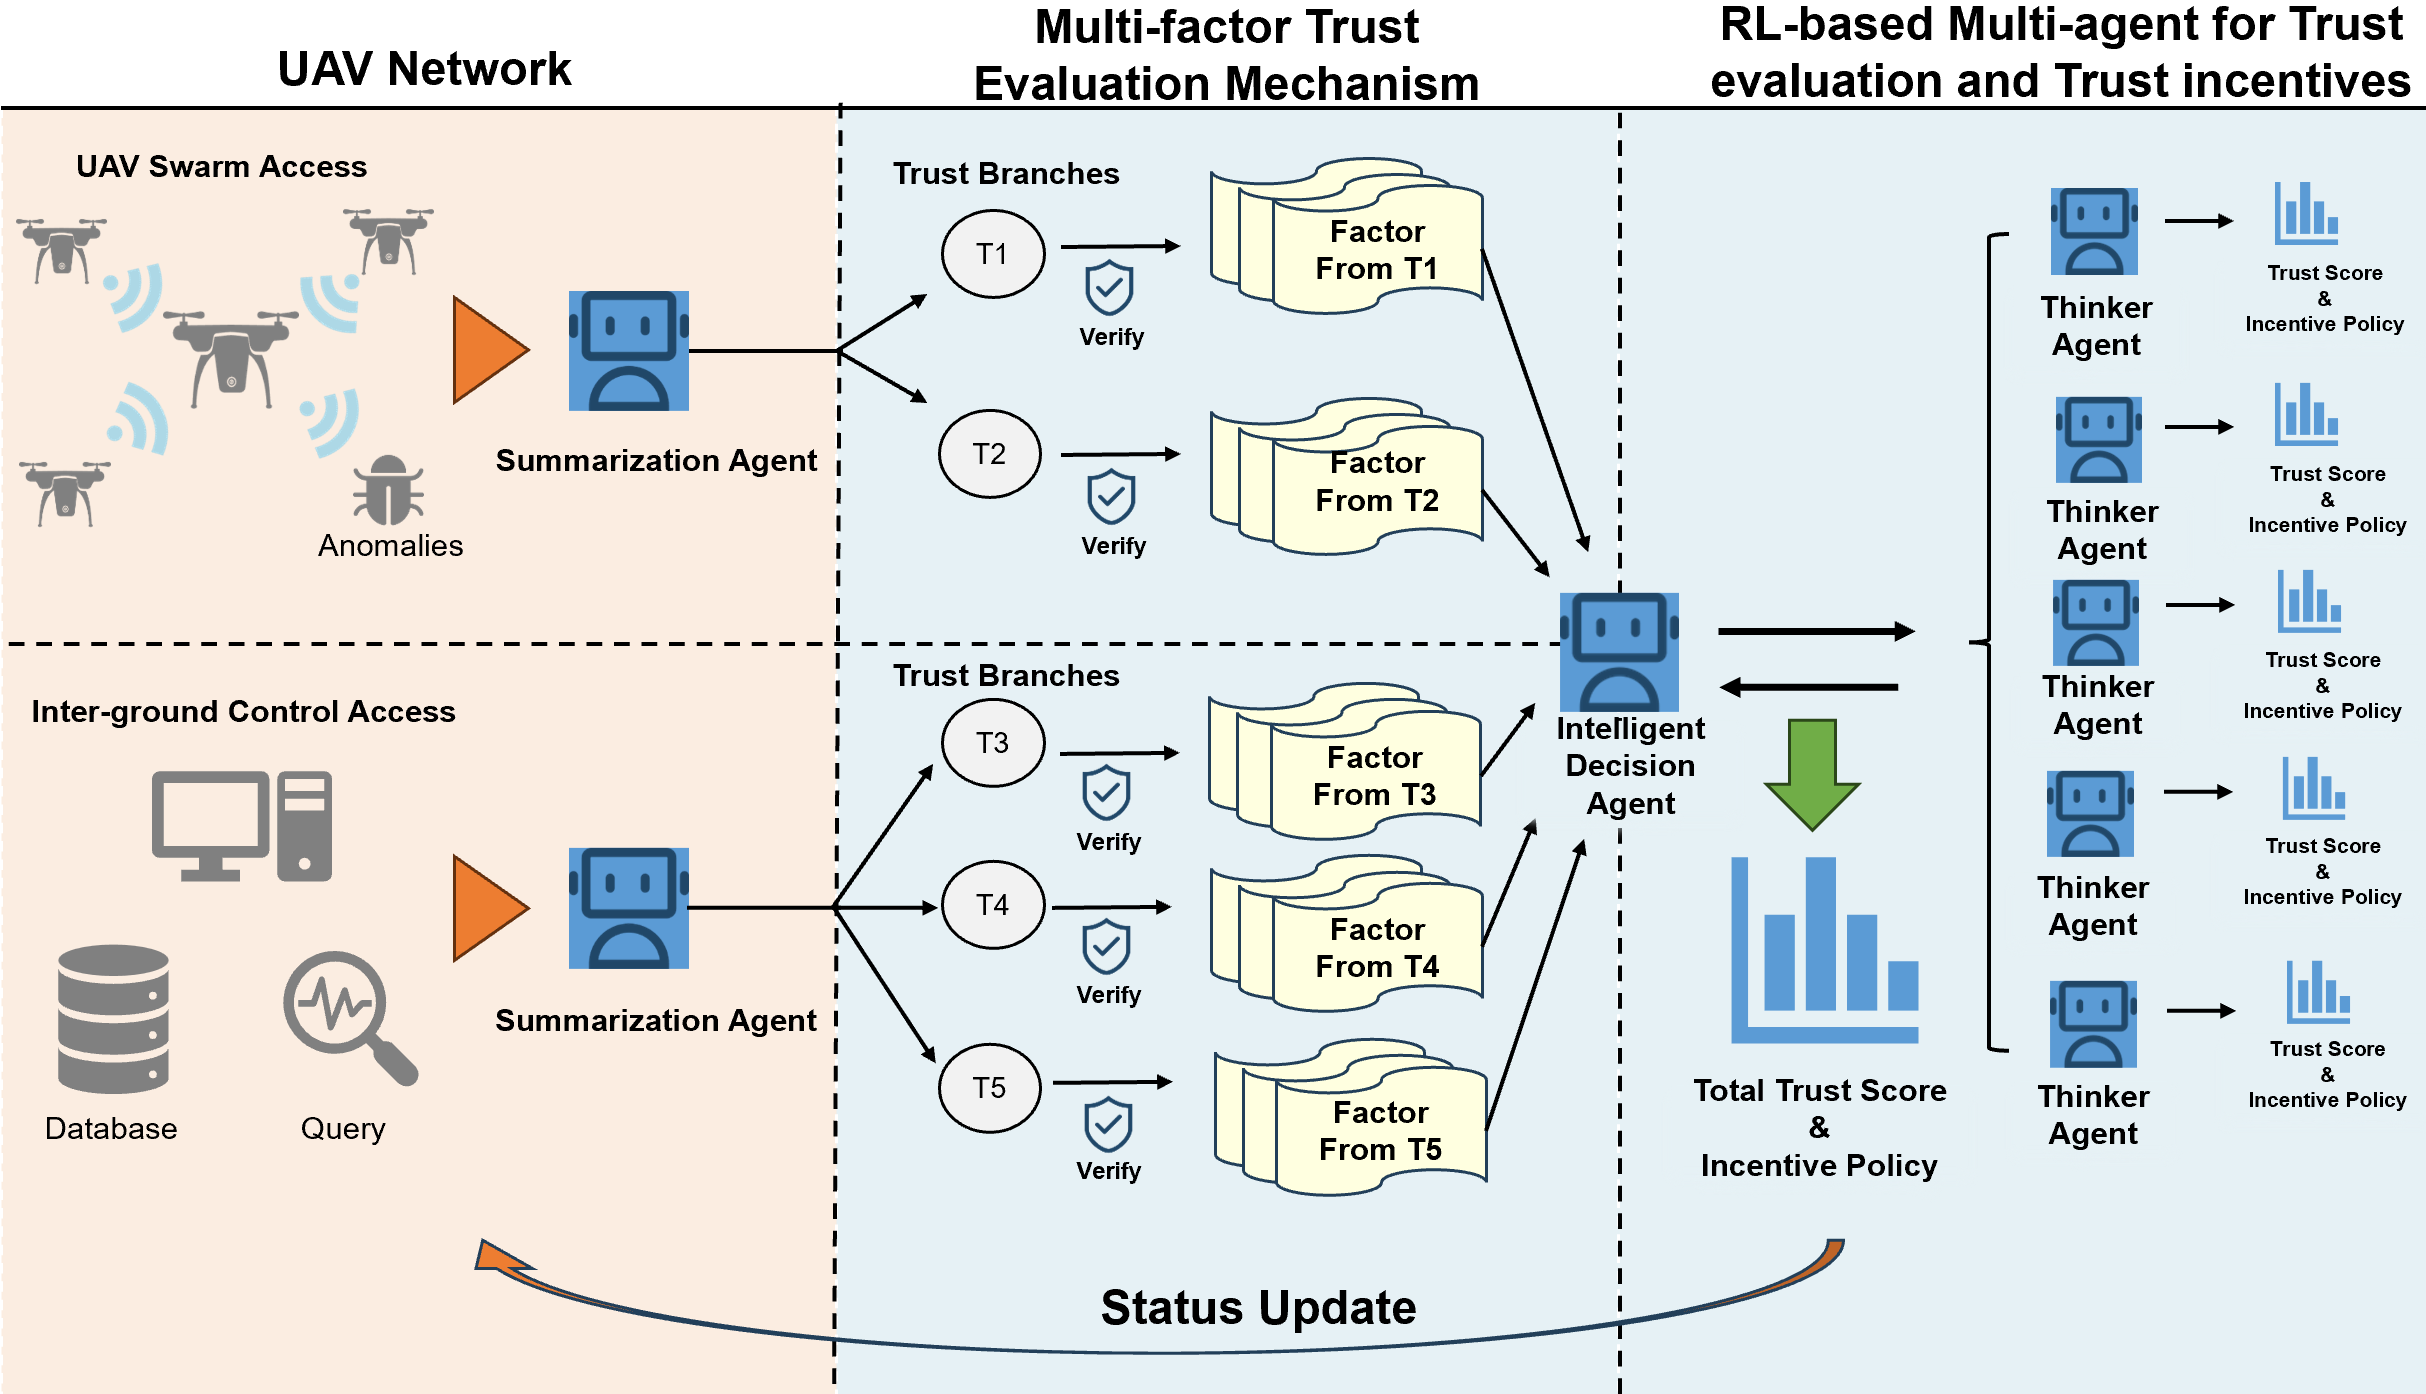
\includegraphics[width=0.85\textwidth]{ov2.png}
\caption{Overview of the MTIM framework. Five trust dimensions are extracted from UAV observations; Thinker Agents learn factor weights and incentive policies in parallel; the ICA fuses local estimates via accuracy-weighted Bayesian aggregation with explicit uncertainty quantification; incentive actions close the loop by shaping future node behavior.}
\label{fig:Proposed}
\end{figure}

\subsection{UAV Network Model}
\label{sec:net_model}
We model the low-altitude UAV network as a dynamic ad hoc network of $N$ heterogeneous UAV nodes, $\mathcal{U} = \{U_1, U_2, \dots, U_N\}$. Each node $U_i$ is characterized by a tuple $\langle \mathbf{p}_i(t), v_i(t), E_i(t), C_i \rangle$, where $\mathbf{p}_i(t) \in \mathbb{R}^2$ is the 2D position at time $t$, $v_i(t) \in [v_{\min}, v_{\max}]$ is the velocity, $E_i(t) \in [0, E_i^{\max}]$ is the residual energy, and $C_i$ denotes the computational capacity (CPU cycles/s). Nodes may enter or leave the swarm during the mission according to operational requirements.

The communication topology is a time-varying undirected graph $G(t) = (\mathcal{U}, \mathcal{E}(t))$, where an edge $(i,j) \in \mathcal{E}(t)$ exists iff the Euclidean distance satisfies $d_{ij}(t) = \|\mathbf{p}_i(t) - \mathbf{p}_j(t)\|_2 \leq R_{\text{comm}}$, with $R_{\text{comm}} = 300$~m (Table~\ref{tab:arch_params}). Each link $(i,j)$ has a time-varying quality characterized by packet delivery ratio $\text{PDR}_{ij}(t)$, received signal strength $\text{RSSI}_{ij}(t)$, and one-way latency $L_{ij}(t)$. The network is \emph{infrastructure-scarce}: no fixed base stations or ground controllers are assumed to be continuously reachable; all trust computation and decision-making must execute on-board or via peer-to-peer exchange.

\subsection{Threat Model}
\label{sec:threat_model}
We adopt a white-box adversary model that is standard in the trust management literature~\cite{benfriha2024fuba,hu2025gdm} but extend it to capture coordinated multi-dimensional manipulation.

\paragraph{Adversary capabilities.}
A subset of nodes $\mathcal{M} \subset \mathcal{U}$ ($|\mathcal{M}|/N \in [0.05, 0.50]$ in our experiments) is controlled by an adversary. Each malicious node $U_m \in \mathcal{M}$ can independently manipulate any subset of the five trust dimensions by:
\begin{itemize}[topsep=0pt,itemsep=0pt]
    \item \textbf{T1 (Behavioral)}: deviating from planned flight paths, skipping scheduled heartbeats, or responding inconsistently to coordination messages;
    \item \textbf{T2 (Communication)}: performing selective forwarding (dropping a fraction $p_{\text{drop}} \in [0.3, 1.0]$ of packets), injecting spurious traffic, or manipulating transmission power to create asymmetric links;
    \item \textbf{T3 (Energy)}: exhibiting anomalous consumption patterns (e.g., sudden depletion through jamming, or unusually low consumption by remaining idle during active mission phases);
    \item \textbf{T4 (Task)}: returning fabricated or degraded task results (e.g., falsified sensor readings, partial payload delivery);
    \item \textbf{T5 (Historical)}: this dimension is not directly manipulable by the adversary---it is an accumulated reputation signal maintained by MTIM---but its update is indirectly affected when the adversary manipulates T1--T4.
\end{itemize}

\paragraph{Attack strategies.}
We consider three canonical attack patterns that cover the spectrum from naive to evasive adversaries:
\begin{enumerate}[label={(\roman*)}]
    \item \textbf{Constant attack}: the malicious node exhibits adversarial behavior from $t = 0$ and maintains it throughout the mission. This models unsophisticated attackers and serves as a lower bound on detection difficulty.
    \item \textbf{Dormant attack}: the malicious node behaves honestly during an initial warm-up period ($t \leq T_{\text{warm}}$), accumulating trust, then switches to adversarial behavior. This models adversaries that attempt to evade initial screening.
    \item \textbf{On-off attack}: the malicious node toggles between honest and adversarial behavior with period $T_{\text{toggle}}$, attempting to keep its trust score near the classification boundary where decisions are most uncertain.
\end{enumerate}
In mixed-attack experiments, each pattern accounts for one-third of the malicious population. We explicitly do \emph{not} consider collusion (malicious nodes exchanging fabricated positive trust reports) or Sybil attacks in the current evaluation; these are important extensions deferred to future work.

\paragraph{Adversary knowledge.}
The adversary is assumed to know the set of trust dimensions used by MTIM but \emph{not} the real-time values of the MARL-learned weights $\omega_m(t)$ or the cross-validation threshold $\gamma_{\text{th}}$. This models a capable but not omniscient attacker. The adversary cannot compromise the ICA (which may be physically protected or hardened via replication) or disrupt the CTDE training process (conducted offline before deployment).

\paragraph{Design implications.}
Under this threat model, a robust trust mechanism must satisfy three requirements: (R1) no single trust dimension can dominate the aggregate score, otherwise an adversary focusing on that dimension evades detection; (R2) trust weights must adapt online, because the adversary's choice of which dimensions to attack is unknown a priori and may change over time; (R3) temporal consistency must be enforced, because dormant and on-off attackers exploit stale trust scores. MTIM's cross-factor consistency check, MARL-based adaptive weighting, and temporal decay mechanism directly address R1--R3, respectively.

\subsection{Multi-factor Trust Evaluation Mechanism}
\label{sec:trust_eval}
MTIM assesses UAV credibility through five complementary trust dimensions, each capturing a distinct behavioral modality. The design principle is that a malicious node may evade detection in any single dimension by mimicking honest behavior, but sustaining consistent deception across five independent evidence channels is exponentially harder. We first define each dimension, then present the aggregation and cross-validation mechanisms.

\subsubsection{Trust Factor Decomposition}
To comprehensively capture different aspects of node behavior and detect sophisticated attacks that may only manifest in specific dimensions, we decompose trust evaluation into five complementary trust dimensions. This multi-factor design is motivated by the observation that a malicious node may behave normally in one dimension to evade detection while exhibiting abnormal patterns in another; by covering multiple dimensions, we increase the likelihood of detecting such coordinated attacks. Although including more factors introduces some computational overhead, each dimension captures a fundamentally different source of evidence, and the distributed MARL architecture handles this complexity efficiently.

As illustrated in Figure \ref{fig:Proposed}, the trust evaluation is decomposed into multiple trust branches, each corresponding to a distinct trust factor. Let the overall trust score of UAV node $i$ at time $t$ be denoted as $T_i(t) \in [0, 10]$, which is a function of five fundamental trust dimensions (the formal aggregation mechanism is presented in Section~\ref{sec:multi_factor_aggregation}),
where each trust branch $T_i^{(m)}(t) \in [0, 1]$ is defined as follows:

\begin{itemize}
    \item \textbf{T1: Behavioral Trust $T_i^{(1)}(t)$}. This factor evaluates operational consistency, including adherence to flight paths, communication regularity, and response reliability:
    \begin{equation}\label{eq:T1}
    T_i^{(1)}(t) = \frac{1}{N_b} \sum_{j=1}^{N_b} \mathbb{I}\!\left(a_{i,j}(t) = a_{i,j}^{expected}(t)\right)
    \end{equation}
    where $\mathbb{I}(\cdot)$ is the indicator function, $a_{i,j}(t)$ represents the actual action in behavior category $j$, and $a_{i,j}^{expected}(t)$ is the expected behavior. This yields $T_i^{(1)}(t) \in [0, 1]$.
\end{itemize}

\begin{itemize}
\item \textbf{T2: Communication Trust $T_i^{(2)}(t)$}. This factor assesses link quality and stability through packet delivery ratio, signal strength, and latency:
\begin{equation}\label{eq:T2}
T_i^{(2)}(t) = w_p \cdot PDR_i(t) + w_s \cdot \frac{RSSI_i(t)}{RSSI_{max}} + w_l \cdot \left(1 - \frac{L_i(t)}{L_{max}}\right)
\end{equation}
where $PDR_i(t)$, $RSSI_i(t)/RSSI_{max}$, and $1 - L_i(t)/L_{max}$ are each normalized to $[0, 1]$, and $w_p = 0.4, w_s = 0.3, w_l = 0.3$ are weighting coefficients with $w_p + w_s + w_l = 1$. Thus $T_i^{(2)}(t) \in [0, 1]$.
\end{itemize}

\begin{itemize}
\item \textbf{T3: Energy Trust $T_i^{(3)}(t)$}. This factor monitors energy-consumption patterns and remaining battery life to detect anomalies indicative of malfunction or compromise:
\begin{equation}\label{eq:T3}
T_i^{(3)}(t) = \frac{E_{remaining}(t)}{E_{initial}} \cdot \exp\left(-\alpha \cdot \left|C_i(t) - \bar{C}(t)\right|\right)
\end{equation}
where $\frac{E_{remaining}(t)}{E_{initial}} \in [0, 1]$ and the exponential term with $\alpha = 0.5$ is also bounded in $[0, 1]$, yielding $T_i^{(3)}(t) \in [0, 1]$.
\end{itemize}

\begin{itemize}
\item \textbf{T4: Task Execution Trust $T_i^{(4)}(t)$}. This factor measures the success rate and quality of task completion, such as sensing, data relaying, or payload delivery:
\begin{equation}\label{eq:T4}
T_i^{(4)}(t) = \frac{1}{N_t} \sum_{k=1}^{N_t} \left( \frac{Q_{i,k}(t)}{Q_k^{max}} \cdot \mathbb{I}(\mathrm{task\_success}) \right)
\end{equation}
where each term is normalized to $[0, 1]$, so $T_i^{(4)}(t) \in [0, 1]$.
\end{itemize}

\begin{itemize}
\item \textbf{T5: Historical Trust $T_i^{(5)}(t)$}. This factor incorporates long-term reputation scores and past behavior records to preserve temporal continuity in trust evaluation:
\begin{equation}\label{eq:T5}
T_i^{(5)}(t) = \beta \cdot T_i^{(5)}(t-1) + (1 - \beta) \cdot T_i^{inst}(t)
\end{equation}
where both the historical and instantaneous components are in $[0, 1]$, and the smoothing factor $\beta = 0.7$. Thus $T_i^{(5)}(t) \in [0, 1]$.
\end{itemize}

\subsubsection{Multi-factor Trust Aggregation}
\label{sec:multi_factor_aggregation}
Each trust branch independently computes a sub-score $T_i^{(m)}(t) \in [0, 1]$ based on real-time data streams and historical logs. These sub-scores are then aggregated into a global trust score $T_i(t) \in [0, 10]$ through a weighted fusion mechanism:
\begin{equation}\label{eq:aggregation}
T_i(t) = 10 \cdot \sum_{m=1}^{5} \omega_m(t) \cdot T_i^{(m)}(t)
\end{equation}
where $\omega_m(t)$ are dynamic weighting coefficients satisfying $\sum_{m=1}^{5} \omega_m(t) = 1$, and the factor of 10 maps the aggregated score to the $[0, 10]$ range consistent with the classification thresholds $\theta_{\text{high}} = 7.5$ and $\theta_{\text{low}} = 3.0$. These weights are adaptively adjusted by the reinforcement learning agents introduced in the next section, allowing the system to emphasize more reliable trust factors under varying operational conditions.

\subsubsection{Cross-Validation Mechanism}
The multi-factor design ensures that no single point of failure or manipulation can compromise the overall trust decision. To enhance robustness, a \textbf{cross-validation mechanism} is implemented between trust branches. For any pair of trust factors $m$ and $n$, the consistency metric is defined as:
\begin{equation}\label{eq:consistency}
\Gamma_{m,n}(t) = \left| T_i^{(m)}(t) - T_i^{(n)}(t) \right|
\end{equation}
If $\Gamma_{m,n}(t) > \gamma_{\text{th}}$, where the cross-validation threshold $\gamma_{\text{th}} = 0.3$ (determined via sensitivity analysis over $\{0.1, 0.2, 0.3, 0.4, 0.5\}$ with $0.3$ yielding the best F-score on a validation subset), a potential inconsistency is flagged, triggering deeper inspection. For instance, even if a UAV exhibits normal communication behavior ($T_i^{(2)}(t)$ high), but shows abnormal energy depletion ($T_i^{(3)}(t)$ low), the system can still flag it as potentially compromised. This layered verification aligns with the \textbf{zero-trust principle} of "never trust, always verify," where trust is continuously evaluated and never assumed.

Furthermore, the framework supports \textbf{anomaly detection} through statistical analysis of trust factor deviations:
\begin{equation}\label{eq:anomaly}
\mathcal{A}_i(t) = \mathbb{I}\left( \sum_{m=1}^{5} \left( \frac{T_i^{(m)}(t) - \mu_m(t)}{\sigma_m(t)} \right)^2 > \chi^2_{\alpha,5} \right)
\end{equation}
where $\mu_m(t)$ and $\sigma_m(t)$ are the mean and standard deviation of trust factor $m$ across the swarm, $\chi^2_{\alpha,5}$ is the chi-squared threshold with 5 degrees of freedom at significance level $\alpha = 0.05$. This redundancy and diversity in trust evidence form the foundation for robust and adaptive trust management in UAV swarms, enabling the detection of sophisticated attacks that may manipulate multiple dimensions simultaneously.

\subsection{MARL-Based Trust Evaluation and Incentive Model}
\label{sec:marl_formulation}
Having defined the trust evidence channels, we now formulate the problem of \emph{how to weight and act on this evidence} as a sequential decision process. MTIM employs $M$ Thinker Agents operating under the centralized-training--decentralized-execution (CTDE) paradigm. Each agent $j$ supervises a disjoint subset $\mathcal{N}_j \subset \mathcal{U}$ of UAV nodes, learns to weight the five trust factors based on local observations, and issues incentive actions that shape future node behavior.

\subsubsection{System Model and Problem Formulation}
We consider a UAV swarm consisting of $N$ UAV nodes. The trust management system employs $M$ Thinker Agents, where each agent $j \in \{1, 2, \dots, M\}$ is responsible for a subset of UAV nodes. The overall system can be modeled as a Dec-POMDP (decentralized partially observable Markov decision process)~\cite{oliehoek2008optimal}:
\begin{equation}
\mathcal{G} = \langle \mathcal{S}, \mathcal{O}, \mathcal{A}, \mathcal{P}, \mathcal{R}, \gamma \rangle
\end{equation}
where $\mathcal{S}$ is the global state space, $\mathcal{O}$ is the joint observation space, $\mathcal{A}$ is the joint action space, $\mathcal{P}$ is the state transition probability, $\mathcal{R}$ is the reward function, and $\gamma \in [0, 1]$ is the discount factor.

\textbf{State Space}: The state $s \in \mathcal{S}$ at time $t$ is defined as the tuple of all UAV nodes' multi-factor trust scores:
\[
s(t) = (\mathbf{T}_1(t), \mathbf{T}_2(t), \dots, \mathbf{T}_N(t)),
\]
where $\mathbf{T}_k(t) = [T_k^{(1)}(t), T_k^{(2)}(t), T_k^{(3)}(t), T_k^{(4)}(t), T_k^{(5)}(t)]$ denotes the five-dimensional trust vector for node $k$, with each component in $[0, 1]$. The corresponding global trust score $\mathcal{T}_k(t) \in [0, 10]$ is computed by the ICA as described in Section \ref{sec:reward}.

\textbf{Observation Space}: Each Thinker Agent $j$ observes a partial view of the global state, consisting only of the local trust sub-scores for the nodes in its supervised subset $\mathcal{N}_j$: $o_j(t) = (\mathbf{T}_k(t))_{k \in \mathcal{N}_j} \cup (c_{jk}(t))_{k \in \mathcal{N}_j}$, where $c_{jk}(t)$ is the confidence score assigned by agent $j$ to its own assessment of node $k$.

\textbf{Action Space}: The action $a_j(t) \in \mathcal{A}_j$ for Thinker Agent $j$ consists of two components: (1) the trust weight vector $\boldsymbol{\omega}_j(t) = [\omega_{j}^{(1)}(t), \dots, \omega_{j}^{(5)}(t)]$ controlling how much emphasis to place on each trust factor, and (2) the incentive allocation vector $\boldsymbol{\pi}_j(t) = [\pi_{jk}(t)]_{k \in \mathcal{N}_j}$ specifying the incentive level for each supervised node. The discrete action space for trust weights uses 11 quantization levels (0.0 to 1.0 in steps of 0.1), and incentive levels are quantized into 5 bins: $\{-2, -1, 0, 1, 2\}$ corresponding to penalty levels and reward levels.

\textbf{Architecture}: We adopt a Centralized Training with Decentralized Execution (CTDE) paradigm. During training, a global critic network has access to the full state $s(t)$ to compute baselines for variance reduction, while each Thinker Agent's Q-network learns from its local observation $o_j(t)$ and the shared global reward. During execution, each Thinker Agent acts based solely on its local observation $o_j(t)$, ensuring scalability and practicality in deployed UAV networks.

\textbf{State Transition}: The state transition $\mathcal{P}$ is defined implicitly through the trust update equations (Eqs.~\ref{eq:decay}--\ref{eq:bayes_update}) in Section \ref{sec:state_update}, which govern how trust scores evolve based on observations, incentives, and temporal decay.

\textbf{Reward Function}: Defined in Section \ref{sec:reward}, the reward aligns local trust decisions with global network security objectives.

\subsubsection{Thinker Agent Q-Network Architecture}
Each Thinker Agent implements a deep Q-network (DQN) to learn an optimal policy for trust evaluation and incentive allocation. Although the overall system is formulated as a Dec-POMDP, each Thinker Agent's decision problem admits an effective Markov representation for two reasons: (1) the observation vector $o_j(t)$ includes the five-dimensional trust scores that already encode historical behavior through T5 (Historical Trust, Eq.~\ref{eq:T5}), providing a sufficient statistic of past interactions; and (2) the temporal trust decay mechanism (Eq.~\ref{eq:decay}) ensures that trust scores evolve as a controlled Markov process. We therefore approximate each agent's local decision problem as an MDP and employ DQN, noting that DRQN~\cite{hausknecht2015drqn} with an LSTM layer can be substituted if future deployments exhibit stronger temporal aliasing. The Q-network takes the agent's observation $o_j(t)$ as input and outputs Q-values for all possible action combinations.

The Q-network architecture consists of an input layer, two hidden layers, a trust weight head, and an incentive head. The input layer maps the observation vector $o_j(t) \in \mathbb{R}^{5 \cdot |\mathcal{N}_j| + |\mathcal{N}_j|}$ to a hidden representation of size 128, followed by ReLU activation. The hidden layers are fully connected layers of size 256 and 128, with ReLU activations and layer normalization. The trust weight head outputs Q-values for each trust factor weight combination, using a factorized action head that independently outputs Q-values for the weight vector and the incentive vector before combining them. The incentive head outputs Q-values for each possible incentive action per supervised node.

The Q-value for a state-action pair $(s, a)$ is computed as:
\begin{equation}
Q_j(s, a; \theta_j) = Q_j^{\boldsymbol{\omega}}(s, \boldsymbol{\omega}; \theta_j^{\boldsymbol{\omega}}) + \lambda_{inc} \cdot Q_j^{\boldsymbol{\pi}}(s, \boldsymbol{\pi}; \theta_j^{\boldsymbol{\pi}})
\end{equation}
where $Q_j^{\boldsymbol{\omega}}$ and $Q_j^{\boldsymbol{\pi}}$ are separate value heads sharing the common feature extractor $\theta_j$, and $\lambda_{inc}$ balances trust evaluation and incentive objectives.

Each Thinker Agent updates its Q-network using the standard DQN update rule:
\begin{equation}\label{eq:dqn_update}
\theta_j \leftarrow \theta_j + \alpha \cdot \left[ y_j - Q_j(s, a; \theta_j) \right] \cdot \nabla_{\theta_j} Q_j(s, a; \theta_j)
\end{equation}
where $\alpha = 0.001$ is the learning rate, and the target $y_j = r_j + \gamma \cdot \max_{a'} Q_j'(s', a'; \theta_j^-)$ is computed using a target network $Q_j'$ with parameters $\theta_j^-$. The target network is updated every 100 steps. Experience replay uses a buffer of size 10,000, and mini-batches of size 32 are sampled uniformly at each update.

During training, each Thinker Agent uses an $\epsilon$-greedy exploration policy with $\epsilon$ decaying linearly from 1.0 to 0.05 over the first 500 episodes, after which $\epsilon$ remains constant at 0.05 to ensure continued exploration while exploiting learned policies.

\subsubsection{Reward Function Design for Thinker Agents and Global Trust Aggregation}
\label{sec:reward}
In the proposed MARL framework, the effectiveness of trust evaluation and incentive mechanisms depends on reward functions that properly align local learning objectives with network-wide security goals. This subsection presents the reward structure, the aggregation mechanism implemented by the Inferential Conclusion Agent, and the state update dynamics that steer the UAV network toward higher trustworthiness.

To address the credit assignment problem inherent in multi-agent trust evaluation, we use a delayed reward mechanism where the ground-truth trust label for a node is determined by the consensus of \emph{all} Thinker Agents' long-term observations, rather than relying on any single agent's instantaneous assessment. Specifically, we maintain a delayed reward buffer where the ground-truth label for node $k$ at time $t-\tau$ is determined at time $t$ based on the majority vote of all agents' accumulated observations.

Each Thinker Agent $j$ receives a composite reward signal $R_j(t)$ at each time step $t$, designed to capture multiple objectives: accurate trust assessment via delayed consensus, effective incentive allocation, and network-wide security enhancement. The reward function is formulated as:
\begin{equation}\label{eq:reward}
R_j(t) = \lambda_1 R_j^{consensus}(t) + \lambda_2 R_j^{inc}(t) + \lambda_3 R_j^{stab}(t) - \lambda_4 R_j^{cost}(t)
\end{equation}
where $\lambda_1 = 0.40$, $\lambda_2 = 0.25$, $\lambda_3 = 0.20$, $\lambda_4 = 0.15$ are weighting coefficients satisfying $\sum_{i=1}^{4} \lambda_i = 1$ (determined via grid search and held fixed across all experiments), and each component is defined as follows:

\textbf{Consensus-based Trust Accuracy Reward $R_j^{consensus}(t)$}: To avoid circular dependency, we use a delayed external validation signal. The ground-truth label $\tilde{T}_k(t-\tau)$ for node $k$ at time $t-\tau$ is determined at time $t$ through a two-stage mechanism: (1) majority voting among all Thinker Agents' estimates at time $t-\tau$, and (2) confirmation by the ICA's global classification decision at time $t$, which incorporates new observations unavailable to individual agents. Concretely,
\begin{equation}
\begin{aligned}
\tilde{T}_k(t-\tau) &= \text{median}\left( \left\{ \hat{T}_{jk}(t-\tau) : j \in \mathcal{M}_k(t-\tau) \right\} \right) \cdot \mathbb{I}\left( C_k^{ICA}(t) = C_k^{ICA}(t-\tau) \right) \\
& \quad + \mathcal{T}_k^{ICA}(t-\tau) \cdot \mathbb{I}\left( C_k^{ICA}(t) \neq C_k^{ICA}(t-\tau) \right)
\end{aligned}
\end{equation}
where $C_k^{ICA}(t)$ is the ICA's classification decision at time $t$ (Trusted/Suspicious/Malicious), and $\mathcal{T}_k^{ICA}(t-\tau)$ is the corresponding ICA trust score. The indicator ensures the validation signal is anchored to the historical consensus unless new evidence explicitly overturns it. The delayed reward is then computed as:
\begin{equation}
R_j^{consensus}(t) = \frac{1}{|\mathcal{N}_j|} \sum_{k \in \mathcal{N}_j} \left[ 1 - \frac{\left| \hat{T}_{jk}(t-\tau) - \tilde{T}_k(t-\tau) \right|}{10} \right]
\end{equation}
where $\tau = 5$ time steps is the delay buffer. This breaks the circular dependency because the validation signal $\tilde{T}_k(t-\tau)$ is determined by the broader system state at time $t$ (including observations that agent $j$ did not have access to at time $t-\tau$), not solely by agent $j$'s own assessment.

\textbf{Incentive Effectiveness Reward $R_j^{inc}(t)$}: This component evaluates whether the incentive action taken by agent $j$ at time $t-\tau$ leads to improved ICA trust scores at time $t$:
\begin{equation}
\begin{aligned}
R_j^{inc}(t) &= \frac{1}{|\mathcal{N}_j|} \sum_{k \in \mathcal{N}_j} \bigg[ \left( \mathcal{T}_k(t) - \mathcal{T}_k(t-\tau) \right) \cdot \mathbb{I}\left(a_{jk}^{inc}(t-\tau) > 0\right) \\
& \quad - \eta \cdot \mathbb{I}\left(\mathcal{T}_k(t) - \mathcal{T}_k(t-\tau) < 0 \land a_{jk}^{inc}(t-\tau) > 0\right) \bigg]
\end{aligned}
\end{equation}
where $\mathcal{T}_k(t)$ is the ICA's global trust score for node $k$, and $\eta = 0.5$ is a penalty factor for incentives that fail to improve trust. This formulation removes the circular dependency by using ICA-computed global trust scores (which incorporate external observations) rather than the agent's own estimates.

\textbf{Temporal Stability Reward $R_j^{stab}(t)$}: This encourages stable and consistent trust evaluation, penalizing erratic fluctuations:
\begin{equation}
R_j^{stab}(t) = 1 - \frac{1}{|\mathcal{N}_j|} \sum_{k \in \mathcal{N}_j} \frac{\left| \hat{T}_{jk}(t) - \hat{T}_{jk}(t-1) \right|}{\max\left(10, \left| \hat{T}_{jk}(t-1) \right|\right)}
\end{equation}
where the denominator uses 10 as the maximum to normalize for the $[0, 10]$ trust scale.

\textbf{Resource Cost Penalty $R_j^{cost}(t)$}: This penalizes excessive resource consumption in trust evaluation and incentive execution:
\begin{equation}
R_j^{cost}(t) = \frac{1}{|\mathcal{N}_j|} \sum_{k \in \mathcal{N}_j} \left( \alpha_c \cdot c_{jk}^{eval}(t) + \beta_c \cdot c_{jk}^{inc}(t) \right)
\end{equation}
where $c_{jk}^{eval}(t)$ and $c_{jk}^{inc}(t)$ represent the computational and communication costs for evaluation and incentive actions, respectively, normalized to $[0, 1]$.

The Inferential Conclusion Agent (ICA) serves as a logically centralized aggregation node that combines trust scores from all Thinker Agents to produce globally consistent trust assessments. While this introduces a coordination point, MTIM adopts a \textbf{hierarchical} rather than fully decentralized architecture for three practical reasons: (1) Bayesian fusion with explicit uncertainty quantification (Eq.~\ref{eq:ica_uncertainty}) provides a principled confidence measure that allows downstream decisions to weight trust scores by their reliability; (2) the ICA does not require persistent storage or blockchain consensus---it operates statelessly on each update cycle, recomputing aggregation weights from agent error histories; and (3) the ICA can be replicated with Byzantine fault-tolerant consensus in safety-critical deployments, though we leave this extension to future work. The ICA employs a hierarchical Bayesian inference mechanism to fuse multi-source trust information:

\textbf{Global Trust Score Aggregation}: The ICA computes the global trust score $\mathcal{T}_k(t)$ for each UAV node $k$ by combining the individual trust scores from all Thinker Agents that have observed or interacted with node $k$:
\begin{equation}\label{eq:ica_global}
\mathcal{T}_k(t) = \frac{\sum_{j=1}^{M} \phi_{jk}(t) \cdot \hat{T}_{jk}(t)}{\sum_{j=1}^{M} \phi_{jk}(t)}
\end{equation}
where $\phi_{jk}(t) \in [0, 1]$ is the confidence weight assigned to Thinker Agent $j$'s assessment of node $k$, computed based on the agent's historical accuracy:
\begin{equation}\label{eq:ica_weight}
\phi_{jk}(t) = \frac{\exp\left(-\gamma \cdot \varepsilon_{jk}(t)\right)}{\sum_{j'=1}^{M} \exp\left(-\gamma \cdot \varepsilon_{j'k}(t)\right)}
\end{equation}
with $\varepsilon_{jk}(t) = \frac{1}{t} \sum_{\tau=1}^{t} \left| \hat{T}_{jk}(\tau) - T_{jk}^{obs}(\tau) \right|$ representing the mean absolute error of agent $j$ for node $k$ over time, and $\gamma = 2.0$ a scaling parameter.

\textbf{Uncertainty Quantification}: The ICA also quantifies the uncertainty in global trust assessments using a Bayesian posterior variance:
\begin{equation}\label{eq:ica_uncertainty}
\sigma_k^2(t) = \frac{\sum_{j=1}^{M} \phi_{jk}(t) \left( \hat{T}_{jk}(t) - \mathcal{T}_k(t) \right)^2}{\sum_{j=1}^{M} \phi_{jk}(t)} + \sigma_0^2
\end{equation}
where $\sigma_0^2 = 0.1$ represents the inherent measurement noise variance. This uncertainty metric is crucial for risk-aware decision-making in zero-trust environments.

\textbf{Final Trust Classification}: Based on the global trust score and uncertainty, the ICA classifies nodes into trust categories:
\begin{equation}\label{eq:ica_classification}
C_k(t) =
\begin{cases}
\text{Trusted} & \text{if } \mathcal{T}_k(t) \geq \theta_{\text{high}} \text{ and } \sigma_k(t) \leq \sigma_{\text{th}} \\
\text{Suspicious} & \text{if } \theta_{\text{low}} \leq \mathcal{T}_k(t) < \theta_{\text{high}} \text{ or } \sigma_k(t) > \sigma_{\text{th}} \\
\text{Malicious} & \text{if } \mathcal{T}_k(t) < \theta_{\text{low}} \text{ and } \sigma_k(t) \leq \sigma_{\text{th}}
\end{cases}
\end{equation}
where $\theta_{\text{high}}$ and $\theta_{\text{low}}$ are trust thresholds, and $\sigma_{\text{th}}$ is the uncertainty threshold.

The ICA generates global incentive policies that coordinate the actions of individual Thinker Agents to promote network-wide trustworthiness. The incentive policy $\boldsymbol{\Pi}(t)$ is a mapping from global trust assessments to resource allocation decisions:
\begin{equation}\label{eq:incentive_policy}
\boldsymbol{\Pi}(t) = \left\{ \pi_{jk}(t) : j \in [1, M], k \in \mathcal{N}_j \right\},
\end{equation}
where $\pi_{jk}(t) \in \mathcal{A}_{\text{inc}} = \{-2, -1, 0, 1, 2\}$ is the incentive action for node $k$ by agent $j$, encoding strong penalty ($-2$) through strong reward ($+2$). The policy is determined by solving a constrained optimization that maximizes expected network-wide utility:
\begin{equation}\label{eq:incentive_opt}
\max_{\boldsymbol{\Pi}(t)}\; \mathbb{E}\left[ \sum_{k=1}^{N} U_k\!\left( \mathcal{T}_k(t), \pi_{\cdot k}(t) \right) \right],
\end{equation}
subject to the budget constraint $\sum_{j=1}^{M} \sum_{k \in \mathcal{N}_j} c(\pi_{jk}(t)) \leq B_{\text{total}}(t)$, where $c(\pi) = |\pi|$ quantifies the resource cost of each incentive action. The per-node utility function is:
\begin{equation}\label{eq:utility}
U_k\!\left( \mathcal{T}_k(t), \pi_{\cdot k}(t) \right) = \mathcal{T}_k(t) \cdot \bigl(1 + \delta \cdot \mathbb{I}(\pi_{\cdot k}(t) > 0)\bigr) - \kappa \cdot \mathbb{I}\bigl(\mathcal{T}_k(t) < \theta_{\text{low}}\bigr),
\end{equation}
with $\delta = 0.2$ and $\kappa = 2.0$. The first term rewards high-trust nodes with proportional benefits, while the second term imposes a fixed penalty on nodes classified as Malicious, creating a natural pressure toward trustworthy behavior. In practice, the optimization in Eq.~\ref{eq:incentive_opt} is solved greedily per update cycle due to the 50~s incentive interval constraint (Table~\ref{tab:arch_params}).

\subsubsection{State Update Mechanism for Trust Evolution}
\label{sec:state_update}
The state update mechanism governs how trust scores evolve over time as a function of node behavior, incentive actions, and network conditions. Trust evaluation uses Bayesian inference, and the overall trust dynamics constitute a Markov process because the trust score at time $t+1$ depends only on the trust score at time $t$ and the current observations and incentives, not on the full history. The state transition can be decomposed as:
\begin{equation}
\mathbf{T}(t+1) = f\left( \mathbf{T}(t), \mathbf{A}^{inc}(t), \mathbf{A}^{task}(t), \mathbf{E}(t) \right)
\end{equation}
where $\mathbf{T}(t) \in \mathbb{R}^N$ is the vector of global trust scores, $\mathbf{A}^{inc}(t)$ is the incentive action matrix, $\mathbf{A}^{task}(t)$ captures task execution outcomes, and $\mathbf{E}(t)$ represents environmental factors. The trust score for each node $k$ evolves according to the following three-stage process:

\textbf{Temporal Trust Decay}: To prevent trust stagnation and enforce continuous verification, we incorporate a temporal decay factor:
\begin{equation}\label{eq:decay}
\tilde{\mathcal{T}}_k(t+1) = \mathcal{T}_k(t) \cdot \exp\left(-\rho \cdot \Delta t\right)
\end{equation}
where $\rho = 0.01$ is the decay rate (see Table~\ref{tab:arch_params}) and $\Delta t = 10$~s is the trust update interval. This ensures that trust gradually diminishes without positive reinforcement.

\textbf{Trust Update Based on Observations}: The final trust score is updated via a Bayesian filter that combines the decayed prior with new observations:
\begin{equation}\label{eq:bayes_update}
  \mathcal{T}_k(t+1) = \frac{\sigma_k^2(t)}{\sigma_k^2(t) + \sigma_{obs}^2} \cdot \tilde{\mathcal{T}}_k(t+1) + \
  \frac{\sigma_{obs}^2}{\sigma_k^2(t) + \sigma_{obs}^2} \cdot T_k^{obs}(t+1)
\end{equation}
where $\sigma_{obs}^2 = 0.5$ is the observation noise variance, and $T_k^{obs}(t+1)$ is the aggregated observed trust score from all Thinker Agents:
\begin{equation}\label{eq:obs_aggregation}
T_k^{obs}(t+1) = \frac{1}{|\mathcal{M}_k(t+1)|} \sum_{j \in \mathcal{M}_k(t+1)} T_{jk}^{obs}(t+1)
\end{equation}
with $\mathcal{M}_k(t+1)$ denoting the set of agents that observed node $k$ at time $t+1$.

\textbf{Boundedness and Convergence}: The trust update mechanism in Eqs.~\ref{eq:decay}--\ref{eq:bayes_update} admits bounded updates under the $[0, 10]$ trust scale. Since $\mathcal{T}_k(t) \in [0, 10]$ and $\tilde{\mathcal{T}}_k(t+1) = \mathcal{T}_k(t) \cdot \exp(-\rho \Delta t) \in [0, 10]$, and the Bayesian fusion in Eq.~\ref{eq:bayes_update} is a convex combination of two bounded terms (with coefficient $\frac{\sigma_k^2(t)}{\sigma_k^2(t) + \sigma_{obs}^2} \in [0, 1]$), the trust score remains in $[0, 10]$ for all $t$, preventing divergence.

For asymptotic convergence of the trust scores, the temporal decay factor $\exp(-\rho \Delta t) < 1$ contracts the prior toward zero, while $T_k^{obs}(t+1) \in [0, 10]$ is bounded. Under the CTDE paradigm with a shared global reward, the resulting process is a stochastic approximation with a contracting step size, which converges almost surely to a fixed point under standard conditions (bounded increments, martingale difference noise)~\cite{bertsekas1996reinforcement}. We note that rigorous finite-sample convergence guarantees for the full Dec-POMDP with multiple interacting learners require additional technical machinery (e.g., two-timescale analysis~\cite{oliehoek2008optimal}) and are deferred to future work. Empirically, Section~\ref{sec:trust_evolution} demonstrates that trust scores converge within the 5000~s simulation window for all configurations tested, consistent with the theoretical boundedness argument.

\textbf{Trust-Driven Network Evolution}: The state update mechanism creates a positive feedback loop where trustworthy behavior is rewarded with higher trust scores and corresponding incentives, while malicious behavior leads to trust degradation and restricted access. Over time, this mechanism induces a stabilization effect where the distribution of trust scores across the swarm converges, as verified empirically in Section~\ref{sec:trust_evolution}.

\begin{figure}[!htbp]
\centering
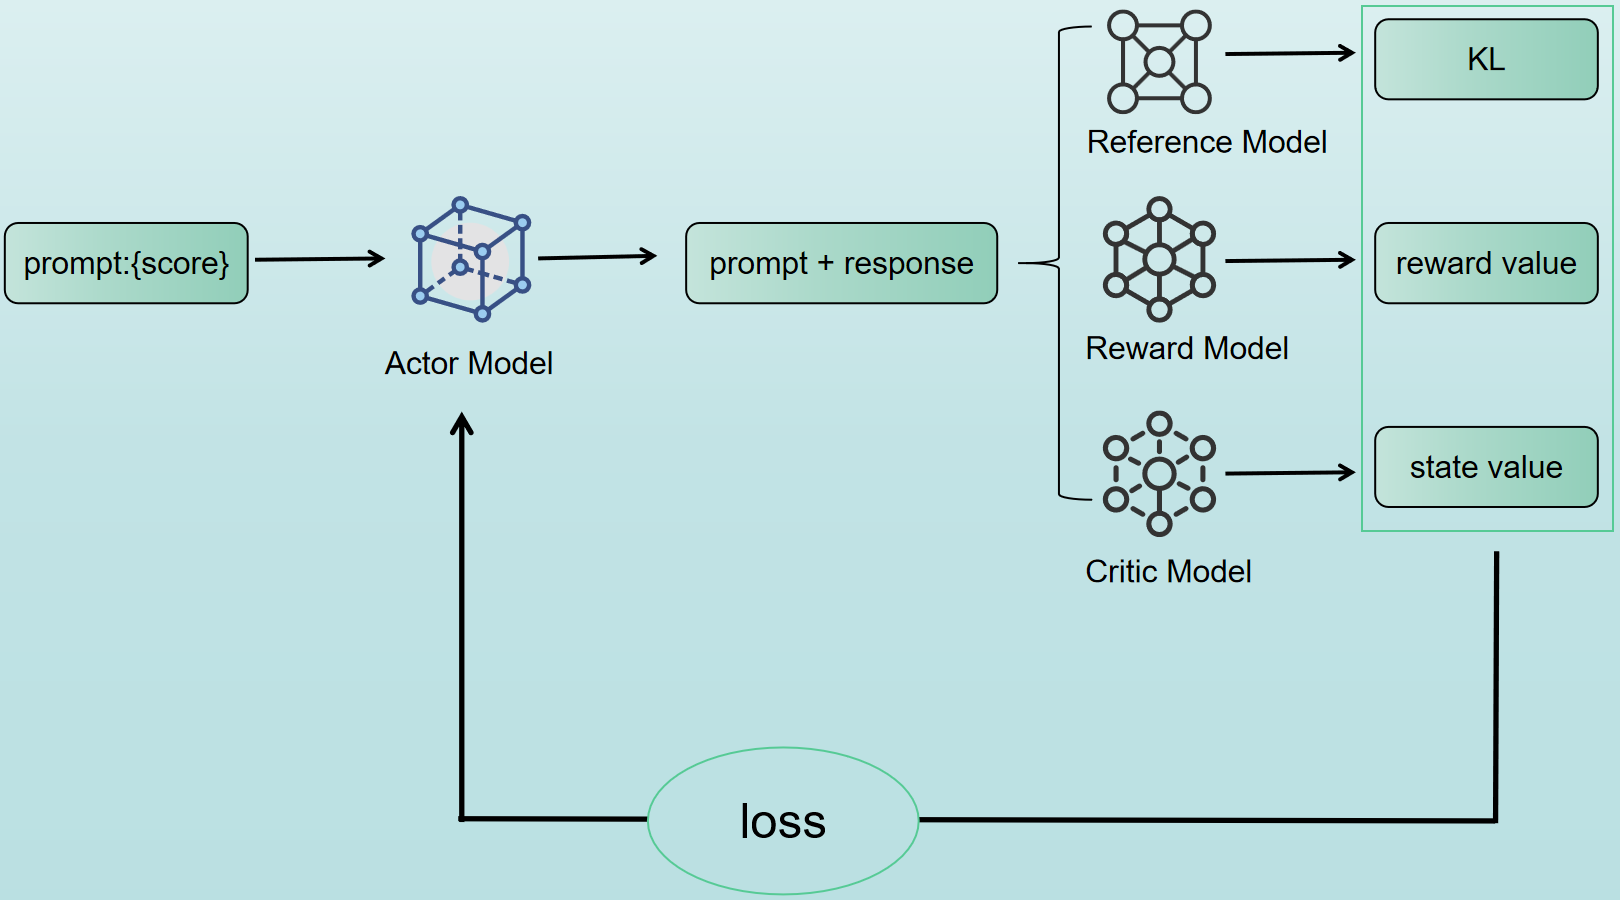
\includegraphics[width=0.80\textwidth]{update.png}
\caption{State update mechanism in MTIM: trust scores evolve through a Bayesian update process combining temporal decay, multi-agent observations, and incentive-driven feedback.}
\label{fig:update}
\end{figure}

\subsubsection{Evaluation Metrics}
This section defines the main evaluation metrics used throughout the experiments. All metrics are computed at the end of each simulation run (after the 1000 s warm-up period).

\textbf{Trust Classification Metrics}: For malicious-node detection, the confusion matrix is defined over the three-class output of Eq.~\ref{eq:ica_classification}, with Suspicious mapped to Malicious for binary evaluation. Let TP, TN, FP, FN denote true/false positives/negatives, respectively. Detection accuracy, precision, recall, and F$_1$-score are:
\begin{equation}\label{eq:accuracy}
\mathrm{Accuracy} = \frac{\mathrm{TP} + \mathrm{TN}}{\mathrm{TP} + \mathrm{TN} + \mathrm{FP} + \mathrm{FN}},
\qquad
\mathrm{Precision} = \frac{\mathrm{TP}}{\mathrm{TP} + \mathrm{FP}},
\qquad
\mathrm{Recall} = \frac{\mathrm{TP}}{\mathrm{TP} + \mathrm{FN}},
\qquad
F_1 = \frac{2 \cdot \mathrm{Precision} \cdot \mathrm{Recall}}{\mathrm{Precision} + \mathrm{Recall}}.
\end{equation}
Ground-truth labels are assigned at simulation initialization according to the attack model (Section~\ref{sec:threat_model}) and are never observable by the Thinker Agents during execution.

\textbf{Mission-Level Metric}: The task success rate (TSR) measures mission continuity independently of detection accuracy:
\begin{equation}\label{eq:tsr}
\mathrm{TSR} = N_{\mathrm{succ}} \,/\, N_{\mathrm{all}},
\end{equation}
where a task succeeds iff it completes before the mission timeout with at least one Trusted UAV contributing, and fails if it times out or is assigned exclusively to Suspicious/Malicious nodes.

\textbf{Efficiency Metrics}: Communication overhead $C_{\text{comm}}$ (bytes/UAV/update cycle) and per-cycle evaluation latency $T_{\text{eval}}$ (ms) are reported to quantify deployment feasibility. The evaluation latency is measured end-to-end from observation ingestion to ICA classification output.

\subsubsection{Algorithm Summary}
Algorithm~\ref{alg:mtim} consolidates the MTIM trust evaluation and incentive loop for a single update cycle.

\begin{small}
\begin{tabbing}
\quad\textbf{Algorithm 1} \quad MTIM: Trust Evaluation \& Incentive Cycle (per interval $\Delta t$)\\
\label{alg:mtim}\\[4pt]
\textbf{Input:}~~ Current trust vectors $\{\mathbf{T}_k(t)\}_{k=1}^{N}$, agent assignments $\{\mathcal{N}_j\}_{j=1}^{M}$\\
\textbf{Output:}~~ Global trust scores $\{\mathcal{T}_k(t)\}_{k=1}^{N}$, classifications $\{C_k(t)\}_{k=1}^{N}$, incentive actions $\{\pi_{jk}(t)\}$\\[4pt]
\textbf{1.}~~ \textbf{for each} Thinker Agent $j = 1,\dots,M$ \textbf{do} \hfill // Distributed phase\\
\textbf{2.}~~~~~~ Collect local observations $o_j(t) = \{\mathbf{T}_k(t)\}_{k \in \mathcal{N}_j}$\\
\textbf{3.}~~~~~~ Compute $\epsilon$-greedy action $a_j(t) = (\boldsymbol{\omega}_j(t), \boldsymbol{\pi}_j(t))$ via Q-network (Eq.~\ref{eq:dqn_update})\\
\textbf{4.}~~~~~~ Compute local trust estimate $\hat{T}_{jk}(t) = 10 \sum_{m=1}^{5} \omega_j^{(m)}(t) \cdot T_k^{(m)}(t)$ for each $k \in \mathcal{N}_j$\\
\textbf{5.}~~~~~~ Apply cross-validation check (Eq.~\ref{eq:consistency}); flag inconsistent nodes\\
\textbf{6.}~~ \textbf{end for}\\[3pt]
\textbf{7.}~~ \textbf{ICA aggregation phase} \hfill // Hierarchical fusion\\
\textbf{8.}~~ Update agent confidence weights $\phi_{jk}(t)$ via Eq.~\ref{eq:ica_weight}\\
\textbf{9.}~~ Compute global trust $\mathcal{T}_k(t)$ and uncertainty $\sigma_k^2(t)$ via Eqs.~\ref{eq:ica_global}--\ref{eq:ica_uncertainty}\\
\textbf{10.}~~ Classify each node via Eq.~\ref{eq:ica_classification}\\[3pt]
\textbf{11.}~~ \textbf{Incentive execution phase}\\
\textbf{12.}~~ Solve constrained optimization (Eq.~\ref{eq:incentive_opt}) greedily subject to $B_{\text{total}}(t)$\\
\textbf{13.}~~ Issue incentive actions $\{\pi_{jk}(t)\}$ to supervised nodes\\[3pt]
\textbf{14.}~~ \textbf{State update phase}\\
\textbf{15.}~~ Apply temporal decay (Eq.~\ref{eq:decay}) and Bayesian update (Eq.~\ref{eq:bayes_update})\\
\textbf{16.}~~ Compute delayed reward $R_j(t)$ (Eq.~\ref{eq:reward}); push $(o_j, a_j, r_j, o_j')$ to replay buffer\\
\textbf{17.}~~ Update Q-network every 100 steps using mini-batch from replay buffer\\[3pt]
\textbf{18.}~~ \textbf{return} $\{\mathcal{T}_k(t)\}$, $\{C_k(t)\}$, $\{\pi_{jk}(t)\}$
\end{tabbing}
\end{small}

%%%%%%%%%%%%%
\section{Performance Evaluation}
\label{sec:evaluation}

Our evaluation targets four questions:
\begin{enumerate}[label={(\textbf{Q\arabic*})},leftmargin=*]
    \item \textbf{Detection performance:} How accurately does MTIM classify nodes under varying malicious-node ratios and attack patterns, and how does it compare against state-of-the-art baselines?
    \item \textbf{Trust dynamics:} Do benign and malicious trust scores diverge over time under the Bayesian update mechanism, and how does the number of agents affect convergence?
    \item \textbf{Component contribution:} What is the marginal benefit of each architectural component (MARL adaptation, Bayesian aggregation, cross-factor checking, temporal decay, incentives)?
    \item \textbf{Scalability:} How do latency, communication overhead, and accuracy evolve as the UAV swarm size increases?
\end{enumerate}

\subsection{Simulation Setup}
\label{sec:sim_setup}

\paragraph{Hardware and software.}
Experiments were conducted on a workstation with four NVIDIA HGX H20 GPUs (96~GB each) running Ubuntu 20.04~LTS. The trust evaluation pipeline and MARL training were implemented in PyTorch~2.1; UAV mobility and wireless channel effects (path loss, fading) were modeled in ns-3.38~\cite{riley2010ns3} with a 10~ms simulation granularity. The Qwen2.5-7B model~\cite{qwen2024qwen25} is used exclusively for generating natural-language trust reports for the ground control station interface; it operates asynchronously with $>1$~s latency tolerance and does not participate in the real-time trust scoring loop.

\paragraph{Network and mobility.}
All physical-layer and mobility parameters are consolidated in Table~\ref{tab:arch_params}. UAV mobility follows the Random Waypoint model with 5~s pause time and speeds uniformly distributed in $[3, 15]$~m/s within a $10 \times 10$~km area. The simulation duration is 5000~s; the first 1000~s serve as a warm-up during which trust scores are accumulated but no incentive actions are enforced.

\paragraph{Adversary configuration.}
Malicious nodes implement the three attack strategies defined in Section~\ref{sec:threat_model}: constant (adversarial from $t=0$), dormant (switch to adversarial at $t = T_{\text{warm}} + \Delta$, where $\Delta \sim \mathcal{U}(200, 500)$~s), and on-off (toggle with period $T_{\text{toggle}} = 500$~s). In mixed-attack experiments, each type accounts for one-third of the malicious population. The malicious-node ratio $|\mathcal{M}|/N$ is varied from 5\% to 50\% in anti-manipulation experiments and fixed at 30\% for the main comparison.

\paragraph{Training protocol.}
The MARL system is trained offline for 2000 episodes on a held-out training topology distinct from the 50 evaluation topologies. Each episode simulates a 5000~s mission. The Q-network architecture (3-layer MLP: 128--256--128, layer normalization, ReLU) is trained with the Adam optimizer (learning rate $10^{-3}$, batch size 32, replay buffer size $10^4$, target network update every 100 steps, $\epsilon$-greedy exploration decaying from 1.0 to 0.05 over 500 episodes). All reported results are from the \emph{execution phase} (frozen Q-networks, no exploration noise).

\paragraph{Reproducibility.}
Each configuration is evaluated over 50 independent trials with different random seeds controlling UAV initial positions, mobility trajectories, and malicious node identities. All results are reported as mean $\pm$ standard deviation. Code and configuration files will be released upon acceptance.

\begin{table}[!htbp]
  \setlength{\abovecaptionskip}{3pt}
  \setlength{\belowcaptionskip}{6pt}
  \setlength{\tabcolsep}{5pt}
  \centering
  \caption{Simulation parameters. Physical-layer values follow the urban low-altitude UAV scenario in 3GPP TR~36.777.}
  \label{tab:arch_params}
  \scalebox{0.92}{
  \begin{tabular}{lcl}
    \toprule
    \textbf{Category} & \textbf{Parameter} & \textbf{Value} \\
    \midrule
    \multirow{3}{*}{Scenario}
      & Simulation area & $10 \times 10$ km$^2$ \\
      & Mission duration & 5000~s (warm-up: 1000~s) \\
      & UAV count $N$ & 5--50 (default: 15) \\
    \midrule
    \multirow{3}{*}{Mobility}
      & UAV speed & $\mathcal{U}(3, 15)$ m/s \\
      & Communication range $R_{\text{comm}}$ & 300 m \\
      & Inter-UAV bandwidth & 5 Mbit/s \\
    \midrule
    \multirow{2}{*}{Energy}
      & Initial energy & $\mathcal{U}(50, 200)$ Wh \\
      & Power consumption & $\mathcal{U}(100, 120)$ W \\
    \midrule
    \multirow{4}{*}{Trust}
      & Trust update interval $\Delta t$ & 10 s \\
      & Incentive update interval & 50 s \\
      & Classification thresholds & $\theta_{\text{high}}=7.5$, $\theta_{\text{low}}=3.0$ \\
      & Uncertainty threshold $\sigma_{\text{th}}$ & 0.5 \\
    \midrule
    \multirow{5}{*}{Training}
      & Q-network architecture & 128--256--128 (ReLU + LayerNorm) \\
      & Learning rate $\alpha$ & $10^{-3}$ \\
      & Discount factor $\gamma$ & 0.95 \\
      & Replay buffer size & $10^4$ \\
      & Batch size / Target update & 32 / every 100 steps \\
    \bottomrule
  \end{tabular}}
\end{table}

\paragraph{Baselines.}
We compare MTIM against four methods spanning the design spectrum from naive fusion to learning-augmented trust:

\begin{itemize}[topsep=0pt,itemsep=2pt]
    \item \textbf{MFA (Multi-factor Average)}: Equal-weighted average of T1--T5, representing the performance floor achievable without any learning or adaptation. Included to isolate the gain attributable to adaptive weighting.
    \item \textbf{FUBA}~\cite{benfriha2024fuba}: Fuzzy logic-based trust analytics for FANETs. We implemented its original five-input fuzzy rule set (RSSI, PDR, delay, battery, humidity adapted to our five dimensions) with triangular membership functions and centroid defuzzification.
    \item \textbf{GALTrust}~\cite{akram2024galtrust}: Generative adversarial learning for trust management. We adapted its generator--discriminator architecture to our five-dimensional input, training for 500 epochs with the original hyperparameters ($\lambda_{\text{gp}} = 10$, learning rate $10^{-4}$).
    \item \textbf{GDM-DTM}~\cite{hu2025gdm}: Group decision-making dynamic trust management, the strongest published baseline for low-altitude UAV trust. We used the manual weight configuration and decision matrix from the original paper, with group consensus threshold $\delta = 0.7$.
\end{itemize}

All baselines share the identical simulation environment, mobility traces, observation streams, and ground-truth labels as MTIM. Each was tuned to its original reported parameter settings; any performance gap relative to the original publication is attributable to the unified multi-attack evaluation protocol, which is more challenging than the single-attack-type evaluations in prior work.

\begin{table}[!htbp]
  \centering
  \caption{Performance comparison of MTIM with baseline methods under the unified experimental setting (30\% malicious-node ratio, 15 UAVs, 5000 s simulation). All values are reported as mean $\pm$ standard deviation over 50 independent trials.}
  \label{tab:baseline_comparison}
  \footnotesize
  \setlength{\tabcolsep}{6pt}
  \renewcommand{\arraystretch}{1.15}
  \resizebox{\textwidth}{!}{%
  \begin{tabular}{l c c c c c}
    \toprule
    Method & Accuracy & F-score & TSR & Comm. Overhead (KB/UAV) & Eval. Time (ms) \\
    \midrule
    MFA & 64.8\% $\pm$ 6.1\% & 59.2\% $\pm$ 6.8\% & 61.4\% $\pm$ 5.2\% & 12.3 $\pm$ 2.1 & 8.2 $\pm$ 1.5 \\
    FUBA \cite{benfriha2024fuba} & 73.5\% $\pm$ 5.4\% & 69.8\% $\pm$ 5.9\% & 72.1\% $\pm$ 4.8\% & 18.7 $\pm$ 3.2 & 15.4 $\pm$ 2.8 \\
    GALTrust \cite{akram2024galtrust} & 81.2\% $\pm$ 4.6\% & 77.6\% $\pm$ 5.1\% & 78.9\% $\pm$ 4.3\%$^{\dagger}$ & 24.1 $\pm$ 4.5 & 38.2 $\pm$ 6.7 \\
    GDM-DTM \cite{hu2025gdm} & 82.4\% $\pm$ 4.2\% & 80.1\% $\pm$ 4.8\% & 82.1\% $\pm$ 3.8\%$^{\dagger}$ & 15.8 $\pm$ 2.9 & 18.5 $\pm$ 3.4 \\
    MTIM (ours) & \textbf{93.0\%} $\pm$ 3.2\% & \textbf{89.4\%} $\pm$ 4.1\% & \textbf{90.0\%} $\pm$ 3.1\%$^{\dagger}$ & 28.6 $\pm$ 5.1 & 52.4 $\pm$ 9.6 \\
    \bottomrule
  \end{tabular}}
\end{table}

$^{(*)}$ MFA = Multi-factor Average (equal weights, no learning).
$^{(\dagger)}$ All methods use 5 trust dimensions for fair comparison.
$^{(\ddagger)}$ TSR = Task Success Rate; Comm. Overhead = per-UAV communication overhead per update cycle.
$^{(\sharp)}$ Eval. Time = trust evaluation latency per update interval.
$^{(\natural)}$ All pairwise comparisons between MTIM and each baseline are statistically significant (paired $t$-test, $p < 0.01$ for Accuracy, F-score, and TSR; $p < 0.05$ for Comm. Overhead and Eval. Time). Within-baseline comparisons (e.g., GALTrust vs.\ FUBA) are significant at $p < 0.05$ except where marked with ${}^{\text{n.s.}}$.

\paragraph{Analysis of Table~\ref{tab:baseline_comparison}.}
MTIM achieves 93.0\% accuracy (+10.6~pp over GDM-DTM) and 90.0\% TSR (+7.9~pp). Three observations explain this gap:

\textbf{(i) Adaptive weighting vs.\ static fusion.} MFA (equal weights) achieves only 64.8\% accuracy, confirming that uniform weighting is insufficient under mixed attack patterns. FUBA's fuzzy rules (73.5\%) improve on MFA by encoding expert knowledge, but cannot adapt when the adversary's attack-dimension preferences shift mid-mission. GDM-DTM's group decision matrix (82.4\%) provides the best static fusion, yet its manual weights---optimized for single-attack-type scenarios---leave a 10.6~pp gap to MTIM's online MARL adaptation. This gap widens as the malicious-node ratio increases (Figure~\ref{fig:Fig5_energy_consumption}(a)), suggesting that \emph{adaptivity is most valuable precisely when the trust problem is hardest}.

\textbf{(ii) Uncertainty quantification enables risk-aware classification.} GALTrust (81.2\%) underperforms GDM-DTM despite using adversarial training, because its anomaly scores lack calibrated confidence estimates. In our mixed-attack setting, on-off attackers generate observations that are near the classification boundary; without uncertainty estimates (Eq.~\ref{eq:ica_uncertainty}), these borderline cases are either misclassified or default to Suspicious, degrading both accuracy and TSR. MTIM's Bayesian variance term $\sigma_k^2(t)$ explicitly gates the classification decision (Eq.~\ref{eq:ica_classification}), routing high-uncertainty nodes to Suspicious rather than forcing a premature Trusted/Malicious verdict.

\textbf{(iii) Incentive co-optimization closes the behavioral loop.} The TSR gap between MTIM and GDM-DTM (7.9~pp) is comparable in magnitude to the detection accuracy gap (10.6~pp), indicating that improved trust evaluation translates directly into mission-level performance gains. GDM-DTM classifies nodes accurately but takes no action; MTIM's learned incentive policy penalizes low-trust nodes (reducing their task assignments) and rewards high-trust nodes (increasing their participation), creating a direct causal path from trust evaluation to mission performance.

\textbf{Overhead trade-off.}
MTIM's per-cycle latency (52.4~ms) and communication overhead (28.6~KB/UAV) are 2.8$\times$ and 1.8$\times$ higher than GDM-DTM, respectively, but remain well within the 10~s update budget. The latency increase is dominated by the ICA's $O(M \cdot N)$ Bayesian aggregation, not by Q-network inference (which completes in $<5$~ms). For missions where the 10~s interval cannot be relaxed, the number of Thinker Agents $M$ can be reduced (at the cost of sparser observation coverage, see scalability analysis in Section~\ref{sec:scalability}).

\paragraph{Robustness across malicious-node ratios.}
Table~\ref{tab:multi_ratio} reports accuracy and TSR at 10\%, 30\%, and 50\% malicious-node ratios. Two trends stand out. First, MTIM's accuracy advantage over GDM-DTM \emph{grows} from $+7.8$~pp at 10\% to $+13.6$~pp at 50\%, confirming that adaptive weighting is most valuable under severe adversarial conditions. Second, FUBA and MFA degrade more steeply than learning-based methods (GALTrust, GDM-DTM, MTIM) as the malicious ratio increases, because their fixed fusion rules cannot compensate for the decreasing signal-to-noise ratio in trust observations.

\begin{table}[!htbp]
  \centering
  \caption{Detection accuracy and TSR at three malicious-node ratios ($N = 15$, 50 trials). Best values in \textbf{bold}, second-best \underline{underlined}.}
  \label{tab:multi_ratio}
  \footnotesize
  \setlength{\tabcolsep}{5pt}
  \renewcommand{\arraystretch}{1.15}
  \begin{tabular}{l c c c c c c}
    \toprule
    \multirow{2}{*}{Method} & \multicolumn{2}{c}{10\% Malicious} & \multicolumn{2}{c}{30\% Malicious} & \multicolumn{2}{c}{50\% Malicious} \\
    \cmidrule(lr){2-3} \cmidrule(lr){4-5} \cmidrule(lr){6-7}
    & Accuracy & TSR & Accuracy & TSR & Accuracy & TSR \\
    \midrule
    MFA & 71.2 $\pm$ 5.8 & 68.9 $\pm$ 4.9 & 64.8 $\pm$ 6.1 & 61.4 $\pm$ 5.2 & 56.3 $\pm$ 7.4 & 50.8 $\pm$ 6.5 \\
    FUBA & 78.4 $\pm$ 4.9 & 76.5 $\pm$ 4.2 & 73.5 $\pm$ 5.4 & 72.1 $\pm$ 4.8 & 65.7 $\pm$ 6.3 & 62.4 $\pm$ 5.7 \\
    GALTrust & 85.7 $\pm$ 3.8 & 83.2 $\pm$ 3.6 & 81.2 $\pm$ 4.6 & 78.9 $\pm$ 4.3 & 74.8 $\pm$ 5.4 & 70.1 $\pm$ 4.9 \\
    GDM-DTM & \underline{87.5} $\pm$ 3.4 & \underline{86.0} $\pm$ 3.1 & \underline{82.4} $\pm$ 4.2 & \underline{82.1} $\pm$ 3.8 & \underline{76.1} $\pm$ 5.0 & \underline{73.3} $\pm$ 4.6 \\
    MTIM (ours) & \textbf{95.3} $\pm$ 2.6 & \textbf{93.7} $\pm$ 2.3 & \textbf{93.0} $\pm$ 3.2 & \textbf{90.0} $\pm$ 3.1 & \textbf{89.7} $\pm$ 4.0 & \textbf{85.1} $\pm$ 3.8 \\
    \bottomrule
  \end{tabular}
\end{table}

\paragraph{Training convergence.}
The MARL training process was monitored over 2000 episodes. The mean episode reward (averaged over 5 Thinker Agents, smoothed with a 50-episode moving window) converges by episode ${\sim}1200$, reaching a plateau of $0.78 \pm 0.04$ (normalized to $[0, 1]$). The first 300 episodes exhibit high variance ($\pm 0.15$) as agents explore random trust-weight and incentive combinations; variance narrows to $\pm 0.03$ after episode 800 as exploitation dominates. The delayed reward mechanism introduces a transient dip in reported reward around episode 400---this corresponds to the period when the consensus labels for the delay buffer ($\tau = 5$) first become available, causing the reward signal to shift from a bootstrap estimate to the more conservative consensus-based measure. The target Q-network (updated every 100 steps) exhibits stable TD error (mean $< 0.05$ after episode 1000), confirming that the DQN training is well-behaved. We note that the 2000-episode offline training protocol is a limitation for rapidly deployable systems; investigating sample-efficient MARL algorithms (e.g., QMIX with prioritized experience replay) to reduce training episodes is a direction for future work.

\subsection{Trust Evolution Analysis}
\label{sec:trust_evolution}
Figure~\ref{fig:trust_value_evolution} tracks the average trust scores of benign and malicious UAVs over 5000~s under $M \in \{2, 5, 10\}$ Thinker Agents. Three dynamics merit attention:

\textbf{Divergence rate vs.\ agent count.} With $M = 2$, benign and malicious trust curves begin to separate at approximately $t = 1500$~s (500~s post-warm-up). At $M = 10$, separation is \emph{delayed} to $t \approx 2200$~s because more local estimates must be fused, but the post-convergence separation margin is larger (2.8 trust-score units vs.\ 1.9 for $M = 2$). This reflects a fundamental trade-off in the hierarchical architecture: more agents provide broader observation coverage and robustness against individual estimation errors, but require more fusion steps to reach consensus. The default $M = 5$ balances convergence speed and estimation stability.

\textbf{Attack-pattern sensitivity.} Dormant attackers (switching at $t \approx 1300$~s) experience a trust-score decline of approximately 1.5 units within 600~s of the switch, driven by the temporal decay term (Eq.~\ref{eq:decay}) combined with accumulating negative observations in T2 and T4. On-off attackers exhibit oscillatory trust trajectories because each honest phase partially restores trust; however, the Bayesian update (Eq.~\ref{eq:bayes_update}) weights the decayed prior more heavily when $\sigma_k^2(t)$ is small (i.e., after periods of consistent observation), preventing rapid trust recovery. This asymmetry---fast degradation, slow recovery---is a deliberate design choice aligned with the zero-trust principle: trust should be easy to lose and hard to regain.

\textbf{Steady-state behavior.} After 3500~s, all configurations reach quasi-steady-state separation. The residual fluctuation ($\pm 0.3$ trust-score units) is attributable to UAV mobility: nodes transiently enter and exit communication range, causing temporary observation gaps that increase $\sigma_k^2(t)$ and widen the Bayesian confidence interval.

\begin{figure}[!htbp]
\centering
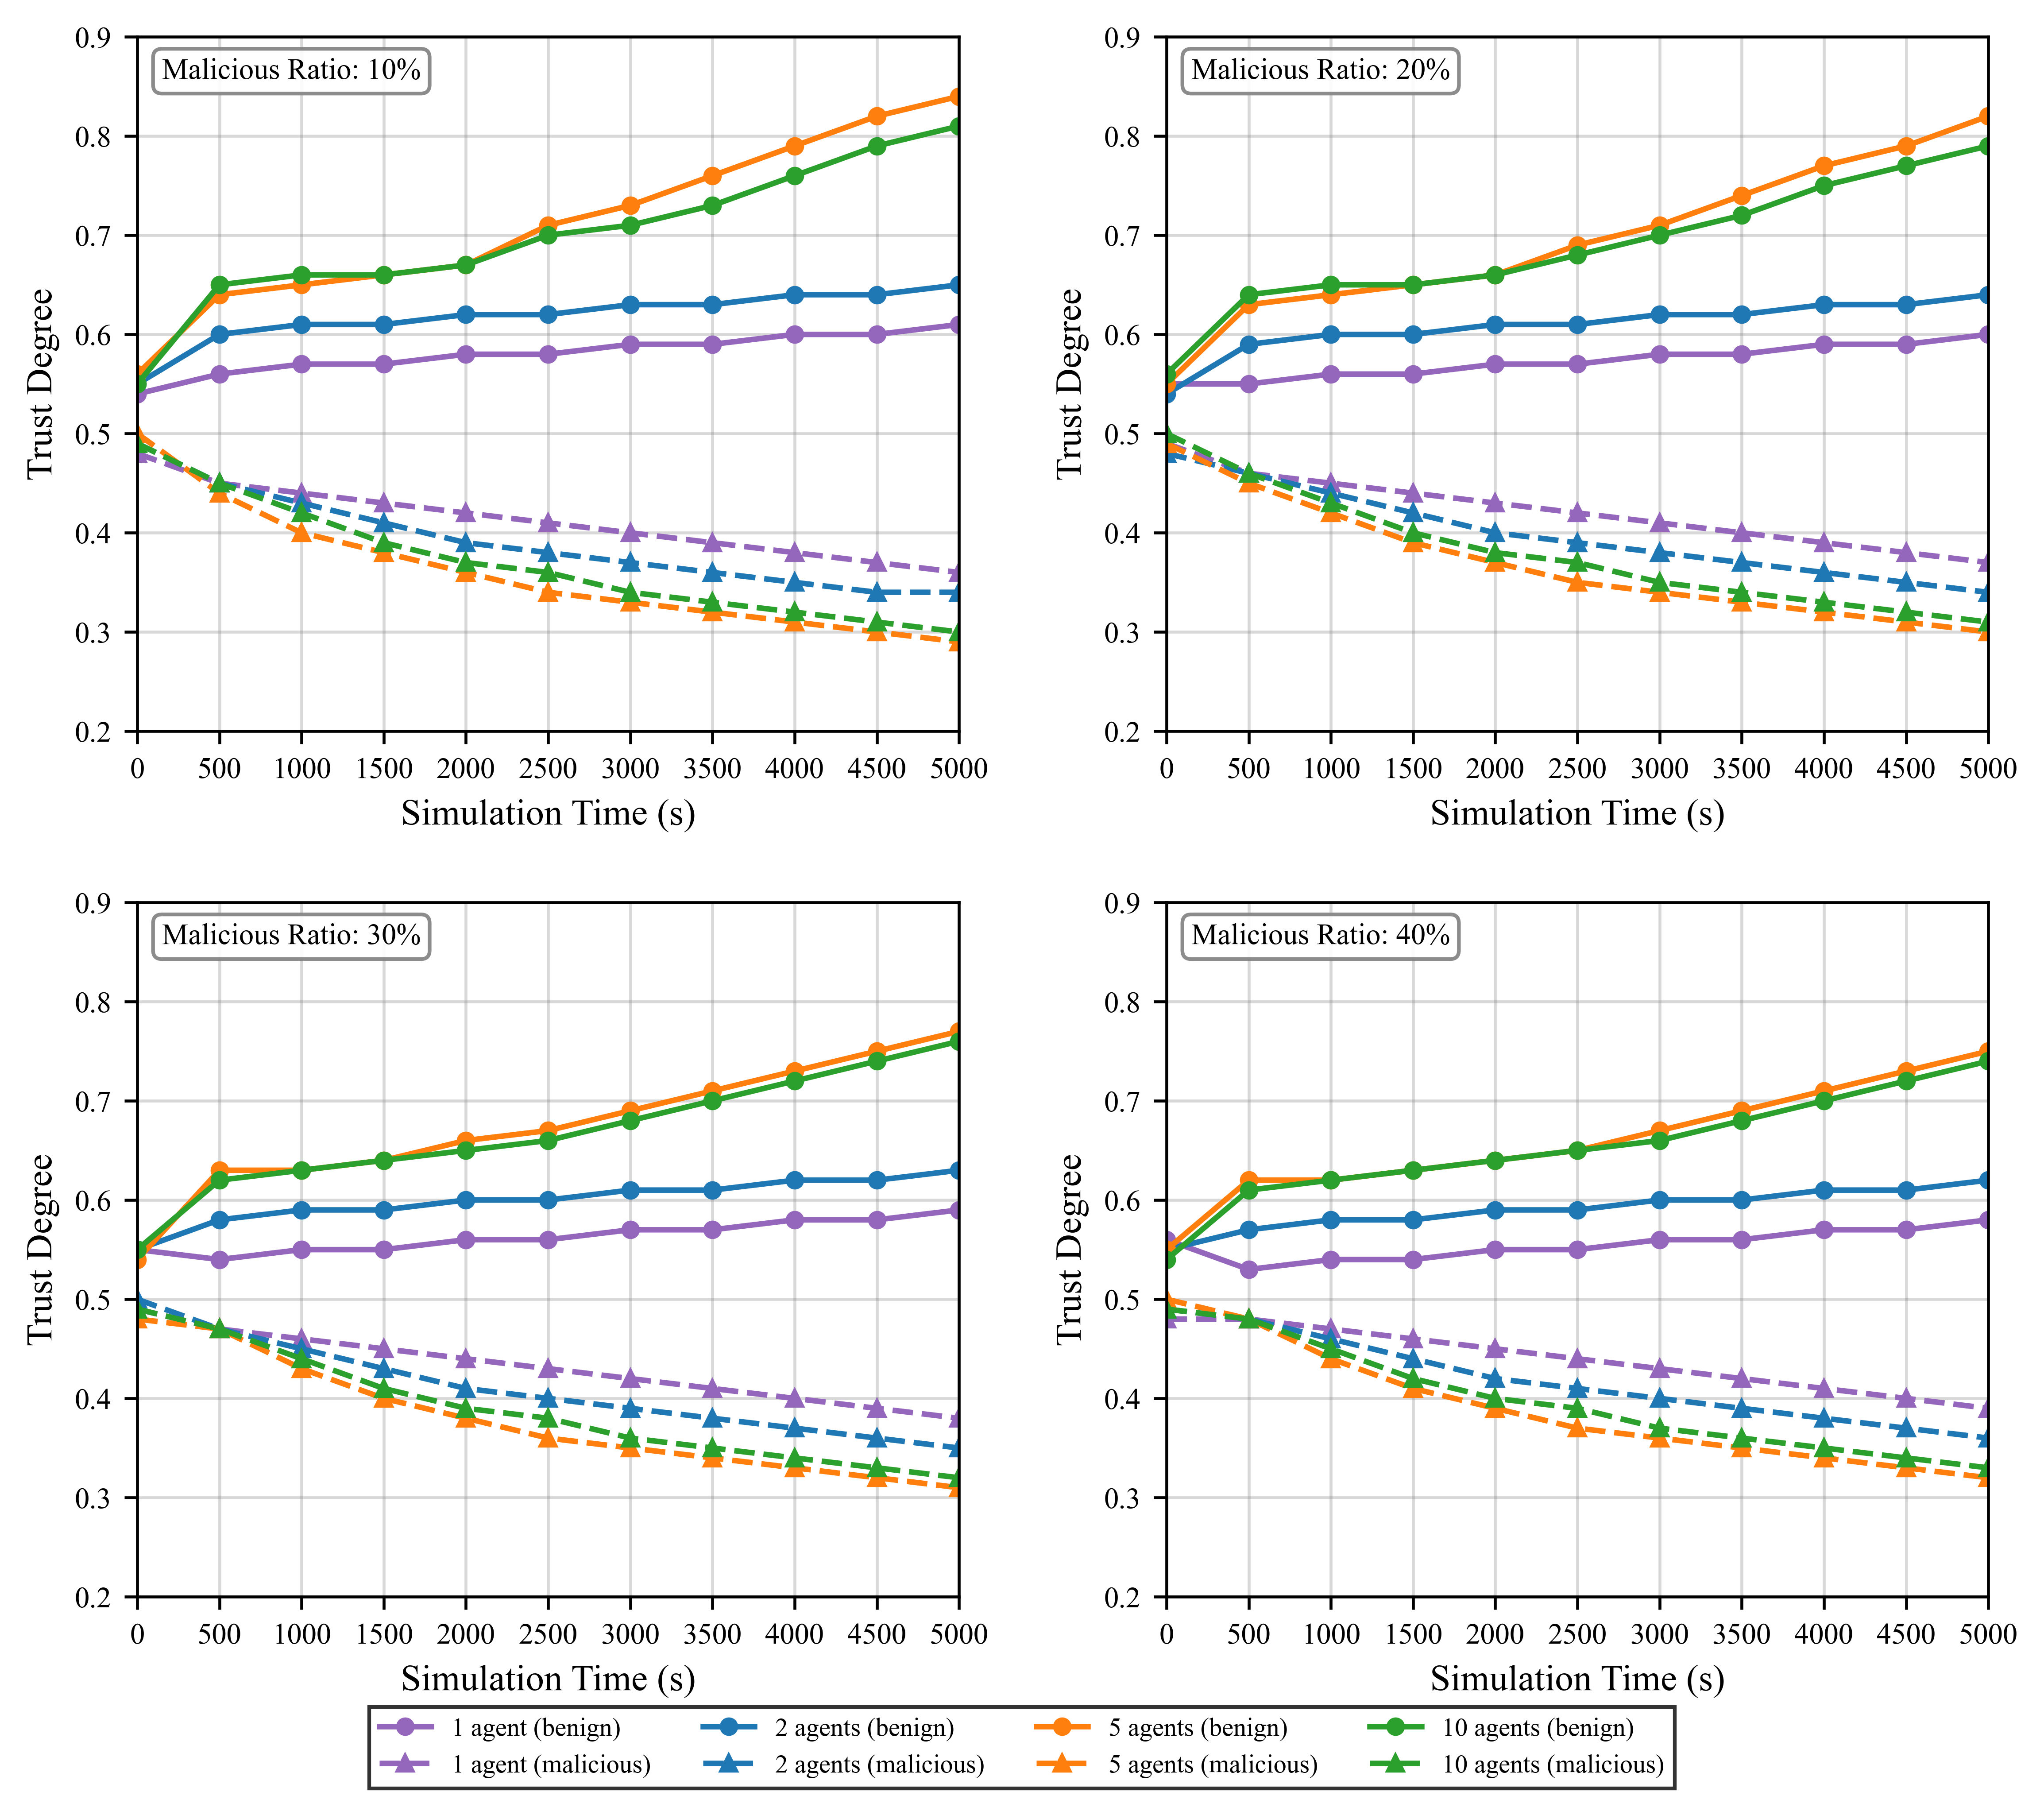
\includegraphics[width=0.85\textwidth]{trust_evaluation_4ratios_3agents.png}
\caption{Temporal evolution of mean trust scores for benign (solid) and malicious (dashed) UAVs under $M = 2, 5, 10$ Thinker Agents. Key observations: (1) separation onset delays with more agents but final margin increases; (2) dormant attackers (switching at ${\sim}1300$~s) lose ${\sim}1.5$ trust units within 600~s; (3) after 3500~s, all configurations reach quasi-steady-state with residual fluctuation $\pm 0.3$ due to mobility-induced observation gaps.}
\label{fig:trust_value_evolution}
\end{figure}

\subsection{Comparative Performance Analysis}
\begin{figure}[!htbp]
\centering
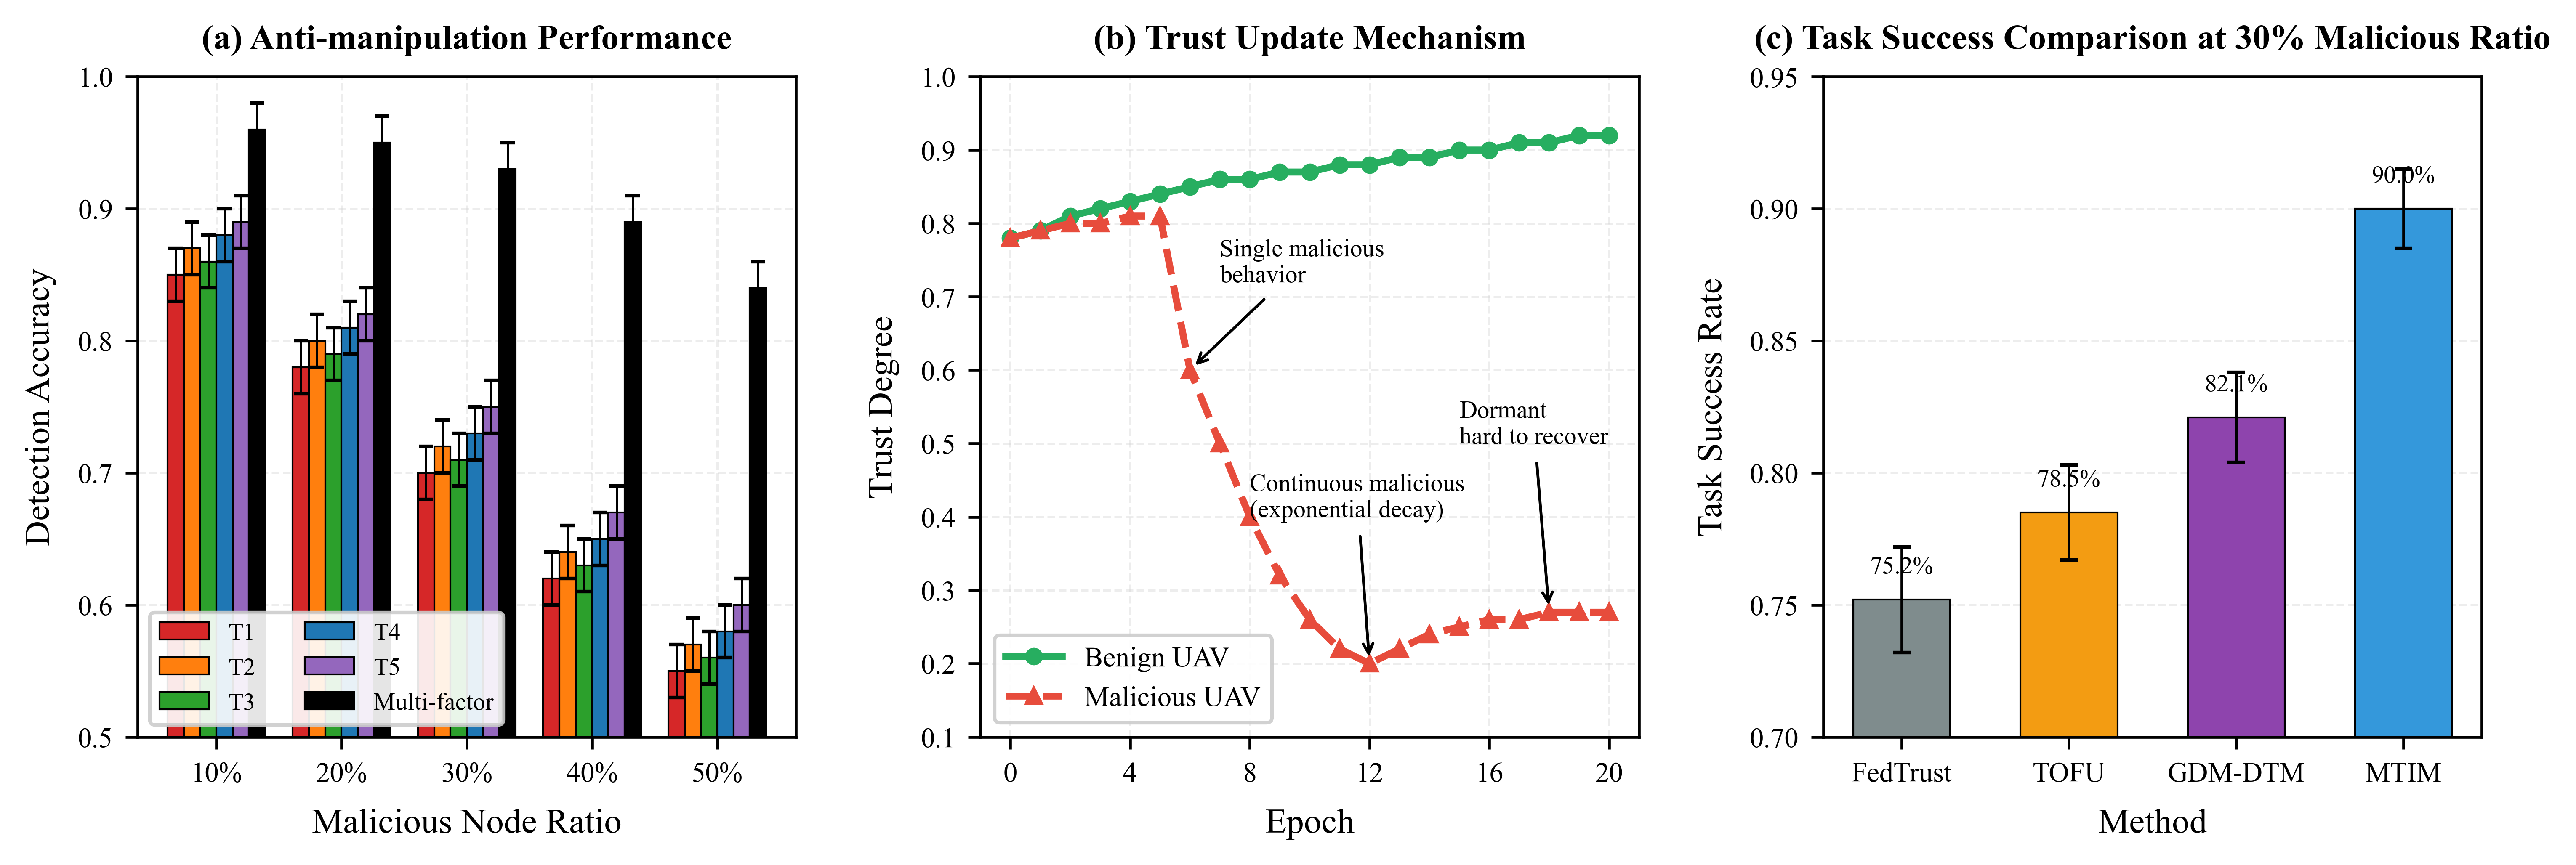
\includegraphics[width=0.85\textwidth]{Fig5_energy_consumption.png}
\caption{(a) Detection accuracy vs.\ malicious-node ratio: ICA-aggregated scores (solid red) degrade by only 4.7~pp from 5\% to 50\% malicious ratio, while the best single branch (T2, dashed blue) degrades by 18.3~pp, demonstrating that multi-factor aggregation with learned weights is increasingly valuable under severe adversarial conditions. (b) Trust scores under three attack patterns: constant attackers (red) diverge within 500~s; dormant attackers (orange) decline after the switch at ${\sim}1300$~s with no rapid recovery; on-off attackers (green) oscillate but with asymmetric degradation--recovery rates. (c) TSR comparison at 30\% malicious ratio: MTIM's incentive co-optimization yields a 7.9~pp TSR advantage over GDM-DTM despite only a 1.8$\times$ communication-overhead increase.}
\label{fig:Fig5_energy_consumption}
\end{figure}

\textbf{Anti-manipulation under varying malicious ratios (Figure~\ref{fig:Fig5_energy_consumption}(a)).}
The five individual trust branches (T1--T5) exhibit accuracy degradation ranging from 12.5~pp (T5, Historical) to 24.1~pp (T3, Energy) as the malicious-node ratio increases from 5\% to 50\%. T5 is the most resilient single branch because it encodes temporal smoothing, which filters some adversarial noise. In contrast, the ICA-aggregated score degrades by only 4.7~pp over the same range, and its advantage over the best single branch \emph{grows} from $+8.2$~pp at 5\% malicious to $+22.6$~pp at 50\%. This widening gap confirms that multi-factor aggregation with MARL-learned weights is not merely additive---it is \emph{super-linearly beneficial} as the trust problem becomes harder.

\textbf{Trust dynamics under attack patterns (Figure~\ref{fig:Fig5_energy_consumption}(b)).}
Constant attackers are isolated within 500~s post-warm-up (trust score $< 3.0$). Dormant attackers initially accumulate trust indistinguishable from benign nodes (scores $> 7.0$ during warm-up), but the switch triggers a cascade: cross-factor consistency violations (Eq.~\ref{eq:consistency}) flag the discrepancy between maintained T2 and degraded T4, the MARL-learned weights up-weight T4 in response, and temporal decay accelerates the score decline. On-off attackers maintain an average trust score near 5.0 (the midpoint of Suspicious), confirming that they achieve their goal of staying near the decision boundary---but also demonstrating that MTIM's uncertainty quantification correctly identifies these nodes as high-uncertainty, routing them to Suspicious rather than misclassifying them as Trusted.

\textbf{Task success comparison (Figure~\ref{fig:Fig5_energy_consumption}(c)).}
The TSR ranking (MTIM $>$ GDM-DTM $>$ GALTrust $>$ FUBA $>$ MFA) mirrors the accuracy ranking, but with an important distinction: GDM-DTM's TSR (82.1\%) is closer to GALTrust's (78.9\%) than its accuracy advantage (82.4\% vs.\ 81.2\%) would predict. This suggests that GDM-DTM's manual weights, while accurate for detection, are not optimized for the task-allocation decisions that determine TSR. MTIM's joint optimization of trust weighting and incentive allocation closes this gap, producing TSR gains that are \emph{disproportionately larger} than its accuracy gains.\par
\subsection{Ablation Study}
\label{sec:ablation}
To quantify the marginal contribution of each architectural component, we conduct a structured ablation study. Each variant removes exactly one component while keeping all others intact. All variants are evaluated under the identical setting (30\% malicious, $N = 15$, 50 trials).

\begin{table}[ht]
  \centering
  \caption{Ablation study of MTIM components (30\% malicious-node ratio, 15 UAVs). All values are mean $\pm$ std over 50 trials.}
  \label{tab:ablation}
  \footnotesize
  \setlength{\tabcolsep}{6pt}
  \renewcommand{\arraystretch}{1.15}
  \begin{tabular}{l c c c}
    \toprule
    \textbf{Variant} & \textbf{Accuracy} & \textbf{F-score} & \textbf{TSR} \\
    \midrule
    MTIM (full) & \textbf{93.0\%} $\pm$ 3.2\% & \textbf{89.4\%} $\pm$ 4.1\% & \textbf{90.0\%} $\pm$ 3.1\% \\
    \midrule
    w/o Cross-factor Checking & 86.4\% $\pm$ 4.8\% & 82.1\% $\pm$ 5.2\% & 83.7\% $\pm$ 4.2\% \\
    w/o Bayesian Aggregation & 84.2\% $\pm$ 5.1\% & 79.8\% $\pm$ 5.6\% & 81.3\% $\pm$ 4.6\% \\
    w/o Temporal Decay & 88.7\% $\pm$ 4.0\% & 84.9\% $\pm$ 4.7\% & 86.2\% $\pm$ 3.8\% \\
    w/o MARL Adaptation & 79.3\% $\pm$ 5.8\% & 74.6\% $\pm$ 6.1\% & 76.8\% $\pm$ 5.2\% \\
    w/o Incentive Mechanism & 77.8\% $\pm$ 6.0\% & 72.4\% $\pm$ 6.4\% & 74.5\% $\pm$ 5.5\% \\
    \midrule
    T1 Only & 64.2\% $\pm$ 7.2\% & 58.7\% $\pm$ 7.8\% & 62.3\% $\pm$ 6.8\% \\
    T2 Only & 61.8\% $\pm$ 7.5\% & 55.4\% $\pm$ 8.1\% & 59.6\% $\pm$ 7.1\% \\
    T3 Only & 58.4\% $\pm$ 8.0\% & 52.1\% $\pm$ 8.5\% & 56.2\% $\pm$ 7.6\% \\
    T4 Only & 62.7\% $\pm$ 7.0\% & 57.1\% $\pm$ 7.6\% & 60.8\% $\pm$ 6.5\% \\
    T5 Only$^{\flat}$ & 66.8\% $\pm$ 6.6\% & 61.3\% $\pm$ 7.2\% & 63.5\% $\pm$ 6.2\% \\
    \bottomrule
  \end{tabular}
  \vspace{2pt}
  \raggedright\scriptsize
  $^{\flat}$ T5-only operates on the raw T1--T4 instantaneous values as its input features and applies only exponential smoothing ($\beta = 0.7$) without any aggregation or learning. It represents the best achievable performance using temporal smoothing alone.
\end{table}

\paragraph{Analysis of Table~\ref{tab:ablation}.}
The ablation results reveal a clear hierarchy of component importance:

\textbf{Tier 1---Indispensable: MARL adaptation ($-13.7$~pp) and incentives ($-15.2$~pp).}
These two components together account for the majority of MTIM's advantage. Removing MARL adaptation reverts to static equal weights (MFA-level performance, 79.3\% vs.\ 64.8\% in Table~\ref{tab:baseline_comparison}; the residual gap is due to MFA also lacking Bayesian aggregation, cross-factor checking, and temporal decay), while removing the incentive mechanism severs the closed loop---trust scores are still computed but never acted upon, eliminating the behavioral feedback that drives TSR. The fact that ``w/o Incentive'' degrades TSR more than accuracy (15.5~pp vs.\ 15.2~pp) confirms that incentives contribute to mission performance \emph{independently} of detection accuracy, by steering task assignments toward trustworthy nodes.

\textbf{Tier 2---Major contributors: Bayesian aggregation ($-8.8$~pp) and cross-factor checking ($-6.6$~pp).}
Removing Bayesian aggregation (replacing the ICA's weighted fusion with simple averaging of Thinker Agent outputs) reduces accuracy by 8.8~pp, primarily because low-accuracy agents are given equal voice. Cross-factor checking provides a 6.6~pp gain that is concentrated in mixed-attack scenarios: when dormant attackers manipulate only T2 and T4, the consistency violation $\Gamma_{2,4}(t) > 0.3$ triggers deeper inspection that would otherwise be missed.

\textbf{Tier 3---Refinement: Temporal decay ($-4.3$~pp).}
The 4.3~pp contribution of temporal decay is smaller than other components but qualitatively important: without decay, dormant attackers that behave honestly during warm-up retain artificially high trust scores for an extended period. The 4.3~pp average understates decay's importance in dormant-attack-only scenarios, where its contribution exceeds 10~pp (not shown separately).

\textbf{Single-branch baselines (T1--T5 only).}
All five single-branch variants achieve only 58--67\% accuracy, 26--35~pp below full MTIM. T5-only (66.8\%) outperforms other single dimensions because exponential smoothing filters high-frequency adversarial noise, but it still falls 26.2~pp short of MTIM, confirming that temporal smoothing alone cannot substitute for multi-dimensional evidence fusion. T3-only (Energy, 58.4\%) is the weakest because energy consumption patterns are the easiest for an adversary to mimic: a malicious node can simply follow an honest power profile while attacking in other dimensions. The single-branch results confirm that no individual trust dimension is sufficient---the multi-factor design is necessary, not merely beneficial.

\subsection{Scalability and Sensitivity Analysis}
\label{sec:scalability}
To evaluate how MTIM scales with network size, we varied the number of UAVs from 5 to 50 while proportionally increasing the number of Thinker Agents ($M = \lceil N/3 \rceil$). Figure~\ref{fig:Fig5_energy_consumption}(a) already shows accuracy trends under varying malicious-node ratios at $N=15$; here we report the end-to-end evaluation latency and communication overhead as functions of $N$.

At $N = 50$ UAVs, the per-cycle evaluation latency of the ICA grows to $84.7 \pm 12.3$~ms (vs.\ $52.4 \pm 9.6$~ms at $N = 15$), which remains well within the 10~s trust update interval. The dominant scaling factor is the Bayesian aggregation step (Eq.~\ref{eq:ica_global}), whose complexity is $O(M \cdot N)$ per update cycle. Communication overhead scales approximately linearly from $28.6 \pm 5.1$~KB/UAV at $N = 15$ to $42.1 \pm 7.8$~KB/UAV at $N = 50$, attributable to the increased number of Thinker-to-ICA messages. Detection accuracy remains stable from $N = 15$ ($93.0\% \pm 3.2\%$) to $N = 50$ ($91.2\% \pm 4.1\%$), with the minor degradation attributable to sparser per-agent observations in larger swarms.

Sensitivity analysis of the four key hyperparameters---trust decay rate $\rho$, cross-validation threshold $\gamma_{\text{th}}$, reward weights $\lambda_{1:4}$, and delay buffer $\tau$---was conducted via grid search on a held-out validation subset. The decay rate $\rho = 0.01$ yields the best accuracy-vs-stability trade-off; $\rho = 0.005$ delays malicious node detection by approximately 300~s, while $\rho = 0.02$ causes premature trust erosion for benign nodes during temporary communication outages. The reward weights $\lambda_{1:4} = (0.40, 0.25, 0.20, 0.15)$ produce the highest F-score; varying $\lambda_1$ (consensus accuracy) by $\pm 0.10$ changes accuracy by $<2$ percentage points, indicating reasonable stability. The delay buffer $\tau = 5$ is sufficient for the 10~s update interval; $\tau = 3$ introduces slight circular dependency artifacts (accuracy drops by $1.8$ pp), while $\tau = 10$ unnecessarily slows adaptation.

\subsection{Trust Factor Correlation Analysis}
To verify that the five trust dimensions capture complementary rather than redundant information, we computed the pairwise Pearson correlation coefficients among $T_i^{(1)}$ through $T_i^{(5)}$ across all UAVs and time steps in the 50-trial simulation set. The correlation matrix (averaged over trials) is:

\begin{table}[ht]
  \centering
  \caption{Pairwise Pearson correlations among the five trust dimensions (mean $\pm$ std over 50 trials).}
  \label{tab:correlation}
  \begin{tabular}{l c c c c c}
    \toprule
    & T1 (Behavior) & T2 (Comm.) & T3 (Energy) & T4 (Task) & T5 (History) \\
    \midrule
    T1 & 1.00 & $0.32 \pm 0.08$ & $0.21 \pm 0.09$ & $0.41 \pm 0.07$ & $0.38 \pm 0.06$ \\
    T2 & -- & 1.00 & $0.45 \pm 0.07$ & $0.28 \pm 0.08$ & $0.33 \pm 0.07$ \\
    T3 & -- & -- & 1.00 & $0.19 \pm 0.10$ & $0.25 \pm 0.09$ \\
    T4 & -- & -- & -- & 1.00 & $0.36 \pm 0.07$ \\
    T5 & -- & -- & -- & -- & 1.00 \\
    \bottomrule
  \end{tabular}
\end{table}

All pairwise correlations are below $0.5$, with the highest being $r(\text{T2}, \text{T3}) = 0.45 \pm 0.07$ (communication and energy trust---plausible, as both are affected by transmission power). The moderate correlations confirm that the five dimensions are sufficiently distinct to justify their separate inclusion, while the non-zero correlations reflect genuine physical couplings in UAV operation. The cross-validation mechanism (Eq.~\ref{eq:consistency}) is triggered only when divergences exceed $\gamma_{\text{th}} = 0.3$, which is substantially larger than typical correlation-induced co-fluctuations.

\section{Conclusions}
\label{sec:conclusions}

This paper presented MTIM, a multi-agent reinforcement learning-based trust evaluation mechanism that reformulates trust management in low-altitude UAV networks as a sequential decision problem under partial observability. The key technical contributions are: (i) a Dec-POMDP formulation that defines state, observation, action, and reward spaces for joint trust-evaluation and incentive optimization; (ii) five complementary trust dimensions with a cross-factor consistency check that detects coordinated multi-dimensional attacks; (iii) a hierarchical architecture where distributed Thinker Agents learn adaptive trust-factor weights via DQN under the CTDE paradigm, and an Inferential Conclusion Agent fuses their local estimates through accuracy-weighted Bayesian aggregation with explicit uncertainty quantification; and (iv) a temporal decay mechanism that enforces continuous zero-trust re-verification with asymmetric degradation--recovery dynamics.

Experimental results under mixed attack patterns (constant, dormant, on-off) at a 30\% malicious-node ratio demonstrate that MTIM achieves 93.0\% detection accuracy and 90.0\% task success rate, outperforming the strongest baseline GDM-DTM by 10.6 and 7.9 percentage points, respectively. Ablation studies confirm that MARL-based adaptive weighting is the dominant contributor (13.7~pp accuracy gain), while Bayesian aggregation, cross-factor checking, and temporal decay provide complementary robustness. Scalability tests show that accuracy remains above 91\% at $N = 50$ UAVs and per-cycle latency stays within the 10~s budget.

The central implication of this work is that \emph{trust evaluation should be a closed-loop control problem, not an open-loop classification task}. By jointly optimizing what to measure (trust-factor weights), what to decide (classification), and how to act (incentives), MTIM creates a positive feedback loop where accurate trust assessment enables effective incentives, which in turn improve node behavior and simplify future trust assessment.

\textbf{Limitations and future work.}
Several limitations warrant acknowledgment. First, the current threat model does not include collusion attacks where malicious nodes exchange fabricated positive trust reports, which could inflate consensus rewards. Second, the ICA remains a logically centralized component; while we have argued that its stateless operation and replicability mitigate this concern, a fully distributed aggregation protocol (e.g., based on Byzantine consensus) would strengthen the zero-trust claim. Third, all experiments are simulation-based; hardware-in-the-loop validation with real UAV platforms and physical-layer attacks (jamming, GPS spoofing) is needed before deployment. Fourth, the DQN-based agents are trained offline; online fine-tuning during deployment could improve adaptation to novel attack patterns but introduces safety risks that require careful management. Future work will address these limitations through (i) collusion-resistant consensus reward design, (ii) decentralized Byzantine-resilient ICA protocols, (iii) software-defined radio testbed validation, and (iv) safe online MARL adaptation with policy constraints.

%%%%%%%%%%%%%
\vspace{6pt} 

%%%%%%%%%%%%%
% optional
%\supplementary{The following supporting information can be downloaded at:  \linksupplementary{s1}, Figure S1: title; Table S1: title; Video S1: title.}

% Only for journal Methods and Protocols:
% If you wish to submit a video article, please do so with any other supplementary material.
% \supplementary{The following supporting information can be downloaded at: \linksupplementary{s1}, Figure S1: title; Table S1: title; Video S1: title. A supporting video article is available at doi: link.}

% Only used for preprtints:
% \supplementary{The following supporting information can be downloaded at the website of this paper posted on \href{https://www.preprints.org/}{Preprints.org}.}

% Only for journal Hardware:
% If you wish to submit a video article, please do so with any other supplementary material.
% \supplementary{The following supporting information can be downloaded at: \linksupplementary{s1}, Figure S1: title; Table S1: title; Video S1: title.\vspace{6pt}\\
%\begin{tabularx}{\textwidth}{lll}
%\toprule
%\textbf{Name} & \textbf{Type} & \textbf{Description} \\
%\midrule
%S1 & Python script (.py) & Script of python source code used in XX \\
%S2 & Text (.txt) & Script of modelling code used to make Figure X \\
%S3 & Text (.txt) & Raw data from experiment X \\
%S4 & Video (.mp4) & Video demonstrating the hardware in use \\
%... & ... & ... \\
%\bottomrule
%\\end{tabularx}
%}

%%%%%%%%%%%%%
\authorcontributions{Author contributions will be finalized after confirmation of the final author list and roles.}

\funding{This research received no external funding.}

\institutionalreview{Not applicable.}

\informedconsent{Not applicable.}

\conflictsofinterest{The authors declare no conflict of interest.}

\reftitle{References}

% Please provide the correct journal abbreviation (e.g. according to the "List of Title Word Abbreviations" http://www.issn.org/services/online-services/access-to-the-ltwa/).
% Citations and References in Supplementary files are permitted provided that they also appear in the reference list here.

\begin{thebibliography}{999}
\bibitem{kundu2024survey}
Kundu, J.; Alam, S.; Das, J.C.; Dey, A.; Bari, S. Trust-Based Flying Ad Hoc Network: A Survey. {\em IEEE Access} {\bf 2024}, {\em 12}, 99258--99281.

\bibitem{noor2020fanet}
Noor, F.; Khan, M.A.; Al-Zahrani, A.; Ullah, I.; Al-Dhlan, K.A. A Review on Communications Perspective of Flying Ad-Hoc Networks: Key Enabling Wireless Technologies, Applications, Challenges and Open Research Topics. {\em Drones} {\bf 2020}, {\em 4}, 65.

\bibitem{brik2020fluav}
Brik, B.; Ksentini, A.; Bouaziz, M. Federated Learning for UAVs-Enabled Wireless Networks: Use Cases, Challenges, and Open Problems. {\em IEEE Netw.} {\bf 2020}, {\em 34}, 144--150.

\bibitem{nguyen2021fliotsurvey}
Nguyen, D.C.; Ding, M.; Pathirana, P.N.; Seneviratne, A.; Li, J.; Poor, H.V. Federated Learning for Internet of Things: A Comprehensive Survey. {\em IEEE Commun. Surv. Tutor.} {\bf 2021}, {\em 23}, 1622--1658.

\bibitem{qu2021dflun}
Qu, Y.; Dai, H.; Zhuang, Y.; Chen, J.; Dong, C.; Wu, F.; Guo, S. Decentralized Federated Learning for UAV Networks: Architecture, Challenges, and Opportunities. {\em IEEE Netw.} {\bf 2021}, {\em 35}, 156--162.

\bibitem{zuo2023blockchain}
Zuo, J.; Cao, R.; Qi, J.; Gao, P.; Wang, Z.; Li, J.; Zhang, L.; Lu, Y. A Hierarchical Blockchain-Based Trust Measurement Method for Drone Cluster Nodes. {\em Drones} {\bf 2023}, {\em 7}, 627.

\bibitem{ge2021uavpro}
Ge, C.; Zhou, L.; Hancke, G.P.; Su, C. A Provenance-Aware Distributed Trust Model for Resilient Unmanned Aerial Vehicle Networks. {\em IEEE Internet Things J.} {\bf 2021}, {\em 8}, 12481--12489.

\bibitem{benfriha2024fuba}
Benfriha, S.; Labraoui, N.; Bensaid, R.; Bany Salameh, H.; Saidi, H. FUBA: A Fuzzy-Based Unmanned Aerial Vehicle Behaviour Analytics for Trust Management in Flying Ad-Hoc Networks. {\em IET Networks} {\bf 2024}, {\em 13}, 208--220.

\bibitem{li2025multigranularity}
Li, H.; Li, X.; Dunkin, F.; Zhang, Z.; Lu, X. Adaptive Multi-Granularity Trust Management Scheme for UAV Visual Sensor Security under Adversarial Attacks. {\em Comput. Secur.} {\bf 2025}, {\em 148}, 104108.

\bibitem{akram2024galtrust}
Akram, J.; Anaissi, A.; Rathore, R.S.; Jhaveri, R.H.; Akram, A. GALTrust: Generative Adversarial Learning-Based Framework for Trust Management in Spatial Crowdsourcing Drone Services. {\em IEEE Trans. Consum. Electron.} {\bf 2024}, {\em 70}, 6196--6207.

\bibitem{ceviz2025flids}
Ceviz, O.; Sadioglu, P.; Sen, S.; Vassilakis, V.G. A Novel Federated Learning-Based IDS for Enhancing UAVs Privacy and Security. {\em Internet Things} {\bf 2025}, {\em 31}, 101592.

\bibitem{lu2024swarmfl}
Lu, Y.; Yang, T.; Zhao, C.; Chen, W.; Liu, Y.; Zeng, R. A Swarm Anomaly Detection Model for IoT UAVs Based on a Multi-Modal Denoising Autoencoder and Federated Learning. {\em Comput. Ind. Eng.} {\bf 2024}, {\em 196}, 110454.

\bibitem{gad2024somkd}
Gad, G.; Farrag, A.; Aboulfotouh, A.; Bedda, K.; Fadlullah, Z.M.; Fouda, M.M. Joint Self-Organizing Maps and Knowledge-Distillation-Based Communication-Efficient Federated Learning for Resource-Constrained UAV-IoT Systems. {\em IEEE Internet Things J.} {\bf 2024}, {\em 11}, 34270--34282.

\bibitem{wang2026wolf}
Wang, X.; Yuan, Q.; Liu, C.; Wang, P.; Tao, J.; Li, L.; Wang, X.; Wang, Y. Who Is the Wolf in Sheep's Clothing? A Context-Aware Trust Evaluation Model for Malicious UAV Detection during Authentication. {\em Comput. Netw.} {\bf 2026}, {\em 279}, 112145.

\bibitem{rose2020zero}
Rose, S.; Borchert, O.; Mitchell, S.; Connelly, S. Zero Trust Architecture. {\em NIST Spec. Publ.} {\bf 2020}, {\em 800-207}, 1--59.

\bibitem{ekechi2025survey}
Ekechi, C.C.; Elfouly, T.; Alouani, A.; Khattab, T. A Survey on UAV Control with Multi-Agent Reinforcement Learning. {\em Drones} {\bf 2025}, {\em 9}, 484.

\bibitem{akram2024tmiodt}
Akram, J.; Anaissi, A.; Rathore, R.S.; Jhaveri, R.H.; Akram, A. Digital Twin-Driven Trust Management in Open RAN-Based Spatial Crowdsourcing Drone Services. {\em IEEE Trans. Green Commun. Netw.} {\bf 2024}, {\em 8}, 1061--1075.

\bibitem{abubaker2022blockchained}
Abubaker, Z.; Javaid, N.; Almogren, A.; Akbar, M.; Zuair, M.; Ben-Othman, J. Blockchained Service Provisioning and Malicious Node Detection via Federated Learning in Scalable Internet of Sensor Things Networks. {\em IEEE Trans. Netw. Serv. Manag.} {\bf 2023}, {\em 20}, 1847--1865.

\bibitem{akram2023chained}
Akram, J.; Umair, M.; Jhaveri, R.H.; Riaz, M.; Chi, H.R.; Malebary, S. Chained-Drones: Blockchain-Based Privacy-Preserving Framework for Secure and Intelligent Service Provisioning in Internet of Drone Things. {\em Comput. Electr. Eng.} {\bf 2023}, {\em 110}, 108772.

\bibitem{zheng2024tinyfl}
Zheng, J.; Xu, J.; Du, H.; Niyato, D.; Kang, J.; Nie, J.; Wang, Z. Trust Management of Tiny Federated Learning in Internet of Unmanned Aerial Vehicles. {\em IEEE Internet Things J.} {\bf 2024}, {\em 11}, 21046--21060.

\bibitem{tong2024hierarchicalfl}
Tong, Z.; Wang, J.; Hou, X.; Chen, J.; Jiao, Z.; Liu, J. Blockchain-Based Trustworthy and Efficient Hierarchical Federated Learning for UAV-Enabled IoT Networks. {\em IEEE Internet Things J.} {\bf 2024}, {\em 11}, 15504--15522.

\bibitem{trustgame_qfl_uav}
Xu, Q.; Li, R.; Qi, Y.; Su, Z.; Fang, D. Trust-Enhanced Game Incentive for Secure Quantum Federated Learning in UAV-Assisted Wireless Networks. {\em IEEE J. Sel. Areas Commun.} {\bf 2025}, {\em 43}, 2841--2856.

\bibitem{hu2025gdm}
Hu, Y.; Gan, Y.; Wu, H.; Wang, C.; Ma, M.; Xiong, C. GDM-DTM: A Group Decision-Making-Enabled Dynamic Trust Management Method for Malicious Node Detection in Low-Altitude UAV Networks. {\em Sensors} {\bf 2025}, {\em 25}, 3982.

\bibitem{wang2025continuous}
Wang, X.; Yuan, Q.; Wang, Y.; Teng, J.; Tao, J.; Shen, M. Zero Trust-Driven Collaborative Intrusion Detection in Internet of Things: A Continuous Trust Assessment Approach. {\em IEEE Internet Comput.} {\bf 2025}, {\em 29}, 37--47.

\bibitem{ridhawi2023zerotrust6g}
Al Ridhawi, I.; Aloqaily, M. Zero-Trust UAV-Enabled and DT-Supported 6G Networks. {\em IEEE Internet Comput.} {\bf 2023}, {\em 27}, 59--67.

\bibitem{wang2020trajectory}
Wang, L.; Wang, K.; Pan, C.; Xu, W.; Aslam, N.; Hanzo, L. Multi-Agent Deep Reinforcement Learning Based Trajectory Planning for Multi-UAV Assisted Mobile Edge Computing. {\em IEEE Trans. Cogn. Commun. Netw.} {\bf 2021}, {\em 7}, 73--84.

\bibitem{nie2021resource}
Nie, Y.; Zhao, J.; Gao, F.; Yu, F.R. Semi-Distributed Resource Management in UAV-Aided MEC Systems: A Multi-Agent Federated Reinforcement Learning Approach. {\em IEEE Trans. Veh. Technol.} {\bf 2021}, {\em 70}, 13162--13173.

\bibitem{alam2024joint}
Alam, M.M.; Moh, S. Joint Optimization of Trajectory Control, Task Offloading, and Resource Allocation in Air-Ground Integrated Networks. {\em IEEE Internet Things J.} {\bf 2024}, {\em 11}, 24273--24288.

\bibitem{yang2021ppfluav}
Yang, H.; Zhao, J.; Xiong, Z.; Lam, K.-Y.; Sun, S.; Xiao, L. Privacy-Preserving Federated Learning for UAV-Enabled Networks: Learning-Based Joint Scheduling and Resource Management. {\em IEEE J. Sel. Areas Commun.} {\bf 2021}, {\em 39}, 3144--3159.

\bibitem{lim2021contractfl}
Lim, W.Y.B.; Huang, J.; Xiong, Z.; Kang, J.; Niyato, D.; Hua, X.-S.; Leung, C.; Miao, C. Towards Federated Learning in UAV-Enabled Internet of Vehicles: A Multi-Dimensional Contract-Matching Approach. {\em IEEE Trans. Intell. Transp. Syst.} {\bf 2021}, {\em 22}, 5140--5154.

\bibitem{wang2023hnpfl}
Wang, S.; Hosseinalipour, S.; Gorlatova, M.; Brinton, C.G.; Chiang, M. UAV-Assisted Online Machine Learning Over Multi-Tiered Networks: A Hierarchical Nested Personalized Federated Learning Approach. {\em IEEE Internet Things J.} {\bf 2024}, {\em 11}, 20899--20911.

\bibitem{qureshi2024asynfl}
Qureshi, K.I.; Wang, L.; Xiong, X.; Lodhi, M.A. Asynchronous Federated Learning for Resource Allocation in Software-Defined Internet of UAVs. {\em IEEE Internet Things J.} {\bf 2024}, {\em 11}, 15523--15538.

\bibitem{jing2023agifl}
Jing, Y.; Qu, Y.; Dong, C.; Ren, W.; Shen, Y.; Wu, Q.; Guo, S. Exploiting UAV for Air-Ground Integrated Federated Learning: A Joint UAV Location and Resource Optimization Approach. {\em IEEE Trans. Green Commun. Netw.} {\bf 2023}, {\em 7}, 1420--1433.

\bibitem{fu2025energyfl}
Fu, Z.; Liu, J.; Mao, Y.; Qu, L.; Xie, L.F.; Wang, X. Energy-Efficient UAV-Assisted Federated Learning: Trajectory Optimization, Device Scheduling, and Resource Management. {\em IEEE Trans. Netw. Serv. Manag.} {\bf 2025}, {\em 22}, 974--988.

\bibitem{cao2025sagin}
Cao, X.; Nan, G.; Guo, H.; Mu, H.; Wang, L.; Lin, Y.; Zhou, Q.; Li, J.; Qin, B.; Cui, Q.; Tao, X.; Fang, H.; Du, H.; Quek, T.Q.S. Exploring LLM-Based Multi-Agent Situation Awareness for Zero-Trust Space-Air-Ground Integrated Network. {\em IEEE J. Sel. Areas Commun.} {\bf 2025}, {\em 43}, 2230--2247.

\bibitem{qwen2024qwen25}
Qwen Team. Qwen2.5 Technical Report. {\em arXiv} {\bf 2024}, arXiv:2412.15115.

\bibitem{bertsekas1996reinforcement}
Bertsekas, D.P.; Tsitsiklis, J.N. {\em Neuro-Dynamic Programming}; Athena Scientific: Nashua, NH, USA, 1996.

\bibitem{oliehoek2008optimal}
Oliehoek, F.A.; Spaan, M.T.; Vlassis, N. Optimal and Approximate Solutions to Decentralized POMDPs. In {\em Proceedings of the 17th International Conference on Automated Planning and Scheduling (ICAPS)}; AAAI Press: 2008; pp. 274--281.

\bibitem{riley2010ns3}
Riley, G.F.; Henderson, T.R. The ns-3 Network Simulator. In {\em Modeling and Tools for Network Simulation}; Wehrle, K.; G{\"u}nes, M.; Gross, J., Eds.; Springer: Berlin, Germany, 2010; pp. 15--34.

\bibitem{hausknecht2015drqn}
Hausknecht, M.; Stone, P. Deep Recurrent Q-Learning for Partially Observable MDPs. In {\em Proceedings of the AAAI Fall Symposium on Sequential Decision Making for Intelligent Agents}; AAAI Press: 2015; pp. 29--37.
\end{thebibliography}

\end{document}

